


\chapter{Review of C}


\section{Goal}

Purpose of this chapter is to review the C language, but with context of embedded programming $\leftrightarrow$ we will focus on features of C which are used in embedded programming (pointer to access registers, bit wise operation,$\cdots$).

\section{Github and Repository}

\underline{Course Repository:} \url{https://github.com/niekiran/Embedded-C/}


\section{GNU tools for windows}

Installing gcc compilter (which is from GNU tools) is not straightforward on windows. The steps are:

\begin{enumerate}
    \item Install the \verb|msys| executable 
    
    \begin{itemize}
        \item Go to \url{https://www.msys2.org/} to install the .exe installer
    \end{itemize}
    
    \item In the command prompt type \verb|msys2|, and it will open an msys shell
    
    \item In the msys shell type the commands:
    
    \begin{enumerate}
        \item \verb|pacman -Syu|
        
        \item \verb|pacman -S --needed base-devel mingw-w64-x86_64-toolchain|
    \end{enumerate}
    
\end{enumerate}


\newpage
\section{Board}

We will use STM32F407G-DISC1 \autoref{fig:Embedded_C:microcontroller_unit}.

\begin{figure}[h]
\centering
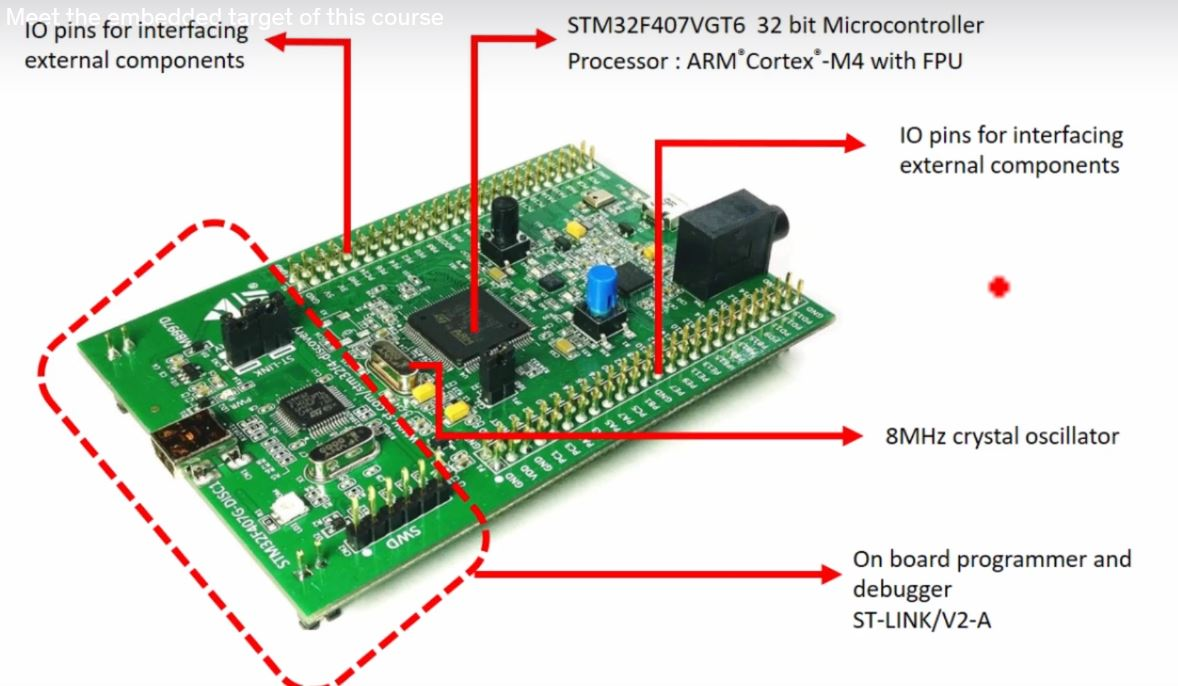
\includegraphics[scale=0.5]{Figures/Embedded_C/microcontroller_unit}
\caption{STM32F407G-DISC1 Main Components}
\label{fig:Embedded_C:microcontroller_unit}
\end{figure}


\subsection{Cable Type}

We also needs usb cable: type A plug to mini type B plug.

\newpage
\section{Creating Project in STMCube IDE}
\label{Sec:creating_project}

In this section we are going to create C projects on 2 type of machines: the host (our computer) and the stm chip (as shown in \autoref{fig:Embedded_C:c_project_types})

\begin{figure}[h]
\centering
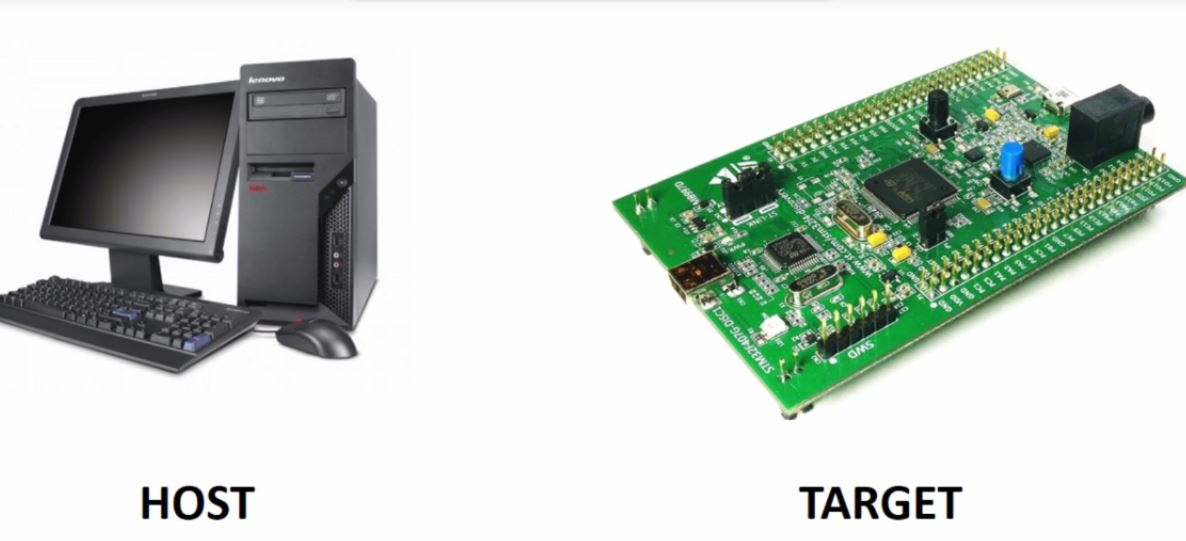
\includegraphics[scale=0.3]{Figures/Embedded_C/c_project_types}
\caption{C Project types: either on a host machine or the embedded target platform}
\label{fig:Embedded_C:c_project_types}
\end{figure}

In StmCube IDE, we need to create $\mathrm{1}^\mathrm{st}$ what is called a  \textit{workspace} for the projects, then we can create the source file codes (\verb|main| file, function,$\cdots$) either for the host or the stm chip. Let's see the steps of creating a workspace first.\\

\subsection{Creating a Workspace}
\label{Sub:creating_workspace}

The steps are:

\begin{enumerate}
    \item We choose some directory (mine is called \verb|Stm32f40g Projects|), and inside the directory we create 2 directory also called: \verb|Host| and \verb|Target|(for the stm)
    
    
    \item We open the IDE, it will give us a prompt to choose the path for the workspace
    
    
    \begin{itemize}
        \item For each type of project (\verb|Host| and \verb|Target|) we create a workspace (so we will have 2 workspace)
    \end{itemize}
    
    \item After we select the path for each workspace, we follow the steps in \ref{sub:creating_project_for_host} or \ref{Sub:Project on Board} 
    
    
\end{enumerate}

Note that when finishing creating a workspace for some directory, we will a \verb|.metadata| folder associated with this workspace.

\subsection{Importing Existing Projects}

Another useful thing to learn is how to import some existing project into our workspace.

This can be useful if for example:

\begin{itemize}
    \item We are cleaning up some existing directory which contains allot of projects, and we need to move them to some new created (clean) directory.\\
    
    This new clean directory will have its own workspace (see \ref{Sub:creating_workspace})
    
    \item Or if we download some new code from others to learn from them, and we need to use them from our code

\end{itemize}

Now concerning the steps for importing an existing projects are:

\begin{enumerate}
    \item Launch the IDE and open to created workspace (this should be created before as discussed in \ref{Sub:creating_workspace})
    
    \item From the tabs, click on \verb|File --> Import|
    
    \item A new window will appear, select on \verb|General --> Existing Project into Workspace|
    
    \item A new window will appear. Using this window we need to do 2 steps:
    
    \begin{enumerate}
        \item From \verb|Select root directory|, browse to the path containing the project (this should lead to root folder containing all the projects)
        
        \item \item In the option, select \verb|Copy project into Workspace|
        
    \end{enumerate}
    

\end{enumerate}



\subsection{Creating a project for Host}
\label{sub:creating_project_for_host}

The steps are:

\begin{enumerate}

    \item Go to \verb|File --> New --> C/C++ Porject|
    
    \item A pop window appear, choose \verb|C Manage Build|
    
    \item Give the project a name
    
    \begin{itemize}
        \item \underline{\textit{Note}:} when giving a name for a source file or a function file, we must include the \verb|.c| extension to STM32Cube IDE (as example :\verb|name_example.c|), so it can create the file
    \end{itemize}
    
    \item Choose from Toolchaine \verb|MinGWGCC| for windows machine (or \verb|LinuxGCC| for Linux machines)
    
    \item Click \verb|Next| then \verb|Finish|
    
    \item A project will appear on the right hand side, then what we do is right click and \verb|New --> source| and give it a name.
    
    \item \underline{Building:} after finishing writing the code, we need to build the project.
    
    Right click on the project name, and select \verb|Build|
    
    \item \underline{Running the project:} right click on the project, select \verb|Run as --> Local C/C++ project|
    
    
\end{enumerate}

\newpage
\subsection{Project on Board}
\label{Sub:Project on Board}

Steps are:

\begin{enumerate}
    \item \verb|File --> New Stm32 Project| 
    
    \begin{itemize}
        \item It will open \textit{Target selection menu} 
    \end{itemize}
    
    \item Select board, and type the stm board name \textit{on the Board Selector menu}
    
    \item Click on Next, then on the project setup, 
    
    \begin{itemize}
        \item Give a name to the project
        
        \item Options: 
        
        Target lanaguage: C
        
        Targeted binary type: executable
        
        Targeted project type: Empty (this is important, we don't select STM32Cube unless we know how to work on smt32cube MX software)
    \end{itemize}
    
\end{enumerate}










\newpage
\section{Data Types in C}

In \autoref{fig:Embedded_C:data_types_C}, we have different data types along with their ranges

\begin{figure}[h]
\centering
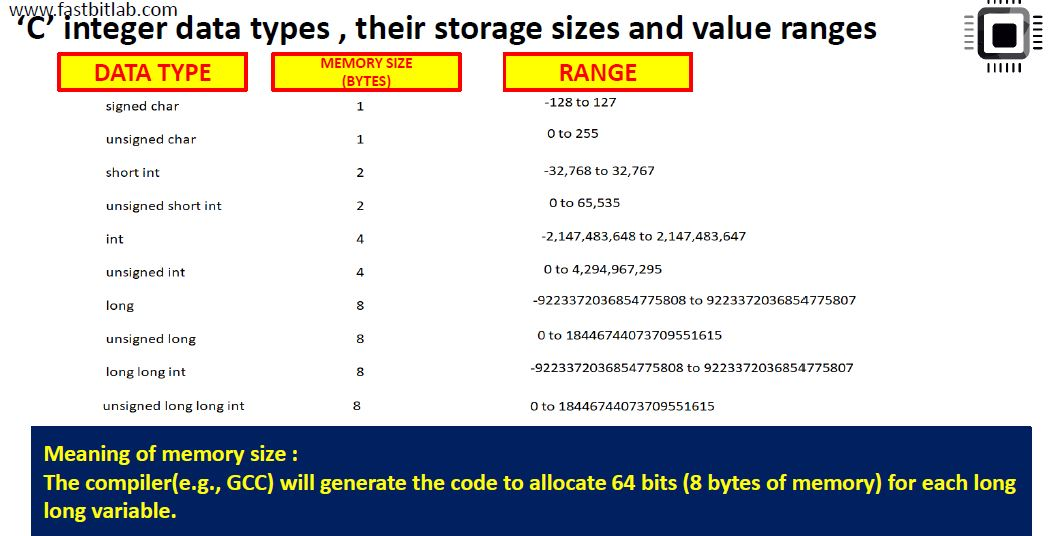
\includegraphics[scale=0.5]{Figures/Embedded_C/data_types_C}
\caption{Data Types in C}
\label{fig:Embedded_C:data_types_C}
\end{figure}

\begin{itemize}
    
\item The important thing is to know that memory sizes are compiler dependent: C standard only specify the max and minimum range, then every compiler designer specify the correspondent size for each data type.

\item However, there are some data types which remains the same for whatever type  of compiler we use

\begin{itemize}
    \item \verb|short int| and \verb|unsigned short int|: consume 2 bytes of memory
\end{itemize}

\end{itemize}


\newpage
\section{Variables in C program}

In C program, variables names are just giving meaning to use as programmer, whereas in the code, the compiler won't use these names, instead it will use \tbi{addresses} to put each variable in its correspondent location with its correspondent value (see \autoref{fig:Embedded_C:variables_C})

\begin{figure}[h]
\centering
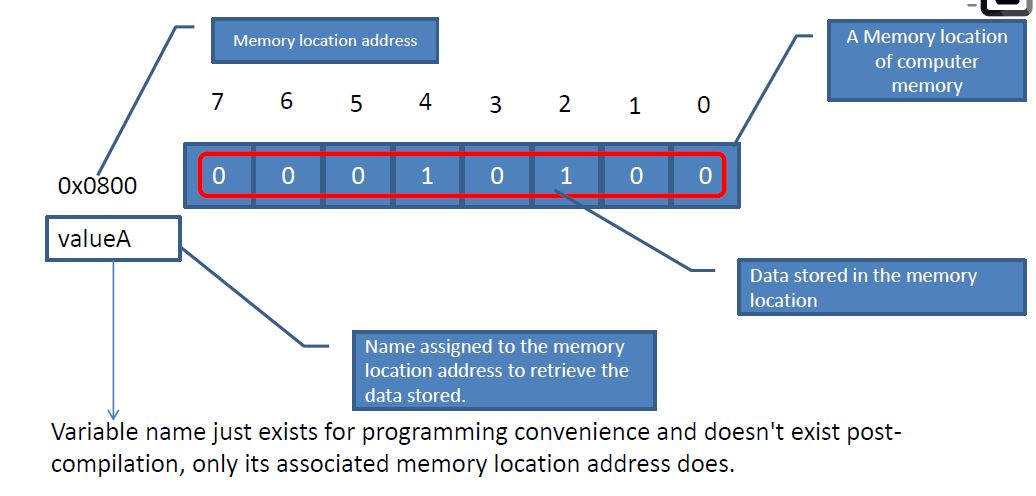
\includegraphics[scale=0.5]{Figures/Embedded_C/variables_C}
\caption{Variables and Memory}
\label{fig:Embedded_C:variables_C}
\end{figure}

\subsection{Declaration Vs Definition}

\begin{itemize}
    \item variable defined $\leftrightarrow$ compiler allocate storage for this variable
    
    \item variable declared $\leftrightarrow$ compiler informed that variable exist but no allocation is done yet (see \autoref{fig:Embedded_C:variables_C_2})
    
    

\begin{figure}[h]
\centering
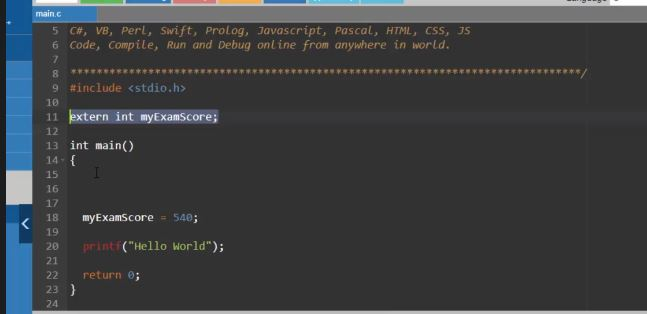
\includegraphics[scale=0.5]{Figures/Embedded_C/variables_C_2}
\caption{Variables and Memory}
\label{fig:Embedded_C:variables_C_2}
\end{figure}  

The \verb|extern| keyword tell the compiler that the variable is defined outside the \verb|main.c| file
    
\end{itemize}


\newpage

\section{Type Casting}

\todo{Casting:} \underline{\textit{Casting}:} \textit{To redo when reviewing the arithmetic system later in logic design}\\

\underline{Big idea:} when not paying attention to data types, we may \tbi{loose information}. Example when doing division between 2 integer, the result will give an integers.

The solution is either:

\begin{enumerate}
    \item Type cast 1 of the variable to float: \verb|float result = (float) int a / int b|
    
    \item Or use directly float data type on the variables \verb|a| and \verb|b|
    
\end{enumerate}

There are also other examples for loss of information when manipulating binary/hex numbers (\textit{to redo them later})

% **********************

\newpage

\section{Hello Stm32}

In this section we will see how to write code on stm32 board.\\

\underline{Note:} Review \autoref{Sub:Project on Board} to create a project.\\

\underline{About the hierarchy of the project:} 

\begin{itemize}
    \item stm32 project include many folder
    
    \begin{itemize}
        \item It will give us an \verb|include| folder where we put our header files, and also a \verb|main.c| file to write our source code
    \end{itemize}
    
    \item Every microcontroller include a \tbi{startup folder}
    
    \begin{itemize}
        \item We will explore the startup code later once we understand more about microcontrollers
    \end{itemize}
    
\end{itemize}

\subsection{Printing Hello world}
\label{Sub:Printing_hello_world}

Now we will try to display a message hello world on the microcontroller. However, we don't have a scree on the STM32F407G-DISC1 (see \autoref{fig:Embedded_C:microcontroller_unit}).\\

The solution for this problem comes from ARM cortex, specifically ARM cortex M3/M4/M7 or higher processors.\\

Let's take a look at \autoref{fig:Embedded_C:swo_pin_st_link}. 

\begin{figure}[h]
\centering
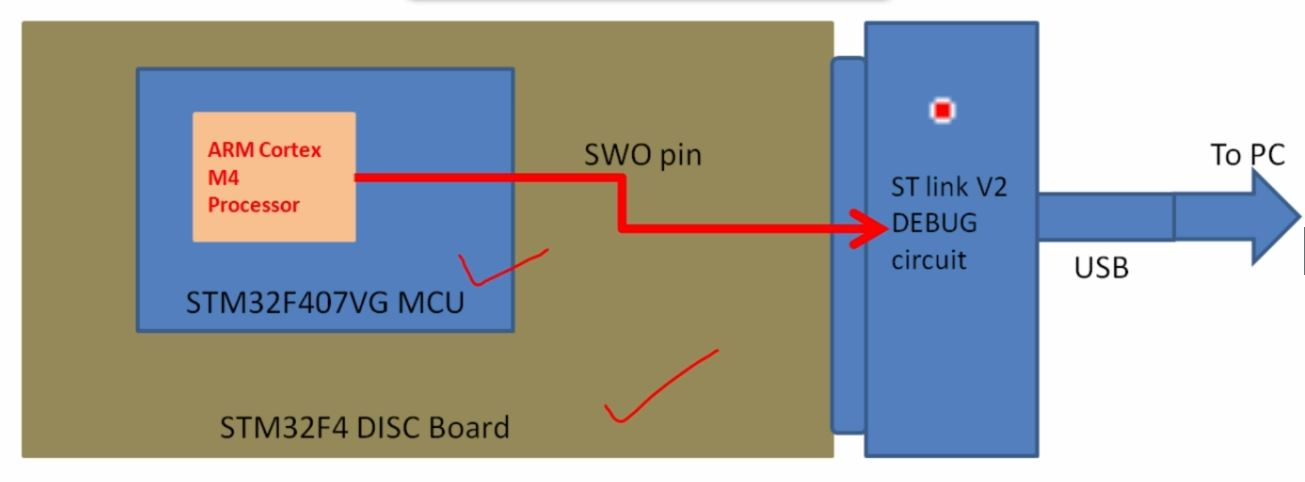
\includegraphics[scale=0.5]{Figures/Embedded_C/swo_pin_st_link}
\caption{Stm discovery board: the SWO pin and st-link debugger}
\label{fig:Embedded_C:swo_pin_st_link}
\end{figure}  

\begin{itemize}
    \item We have the Stm discovery board, and inside the board we have the ARM processor
    
    \item At the front end of the board, we have what we call \tbi{st-link}: this is a circuitry in which we use to communicate our pc/programm to the micronctroller.
    
    Through the st-link, we can write program to the internal flash of the mircrontroller, read various memory location from the mircrontoller, make the micro run and stops.
    
    All debug action are done via the st-link debug circuitry.
    
    \item The st-link debug circuitry talks to our pc through a USB connection
    
    
\end{itemize}

Now we will zoom in inside the ARM cortex M4 only, shown in \autoref{fig:Embedded_C:swo_pin_st_link_zoomed}.

\begin{figure}[h]
\centering
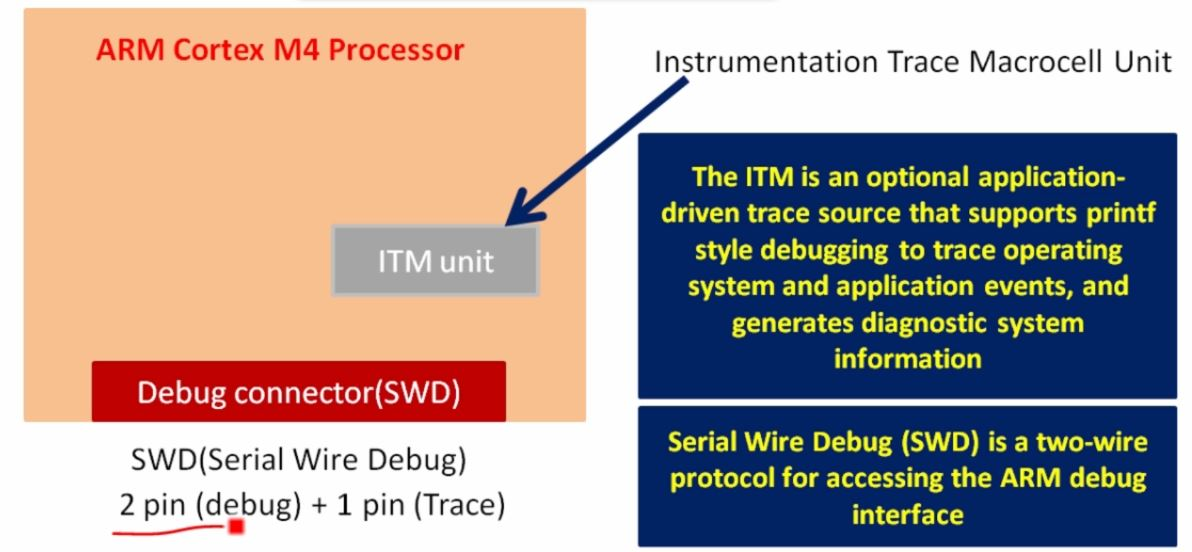
\includegraphics[scale=0.5]{Figures/Embedded_C/swo_pin_st_link_zoomed}
\caption{Stm discovery board: ARM cortex zoomed}
\label{fig:Embedded_C:swo_pin_st_link_zoomed}
\end{figure}  


\begin{itemize}
    \item We have 2 units: the ITM unit and the debug interface, \textit{SWD interface}
    
    \item The SWD interface: it is a debug interface which consists of 2 lines:
    
    \begin{itemize}
        \item The SWDIO line: bidirectional line responsible for the debug information (like when putting a break point,$\cdots$)
        
        \item The SWCLK: a clock driven by the host.  In  our case, the host is the st-link debug circuitry
    \end{itemize}
    
\end{itemize}

\newpage
\underline{Understanding the printf tracing debugging:}\\

Now in order to understand how the \verb|printf| for debugging works, \autoref{fig:Embedded_C:swo_pin_st_link_print} shows the steps:

\begin{figure}[h]
\centering
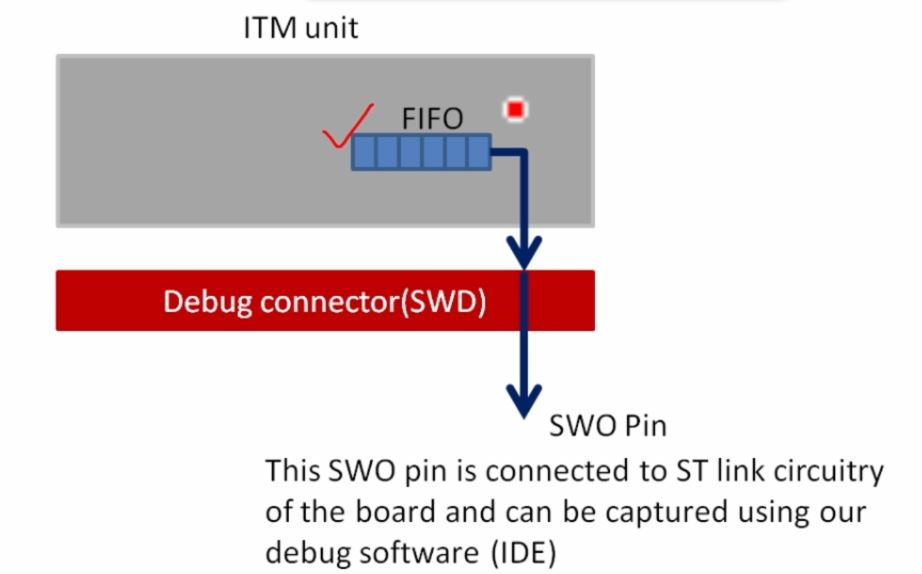
\includegraphics[scale=0.5]{Figures/Embedded_C/swo_pin_st_link_print}
\caption{Stm discovery board: ARM cortex zoomed}
\label{fig:Embedded_C:swo_pin_st_link_print}
\end{figure}  


\begin{itemize}
    \item The data inside the \verb|printf| will go inside the ITM unit, using the FIFO register/buffer
    
    \item Then it will be communicated using the SWO pin, which in turn connected to the ST-link and it will be captured by the IDE
\end{itemize}

\newpage
\underline{Note:} after creating the project, we need to go to  and insert the code in \verb|Src --> syscall.c|.

\begin{figure}[h]
\centering
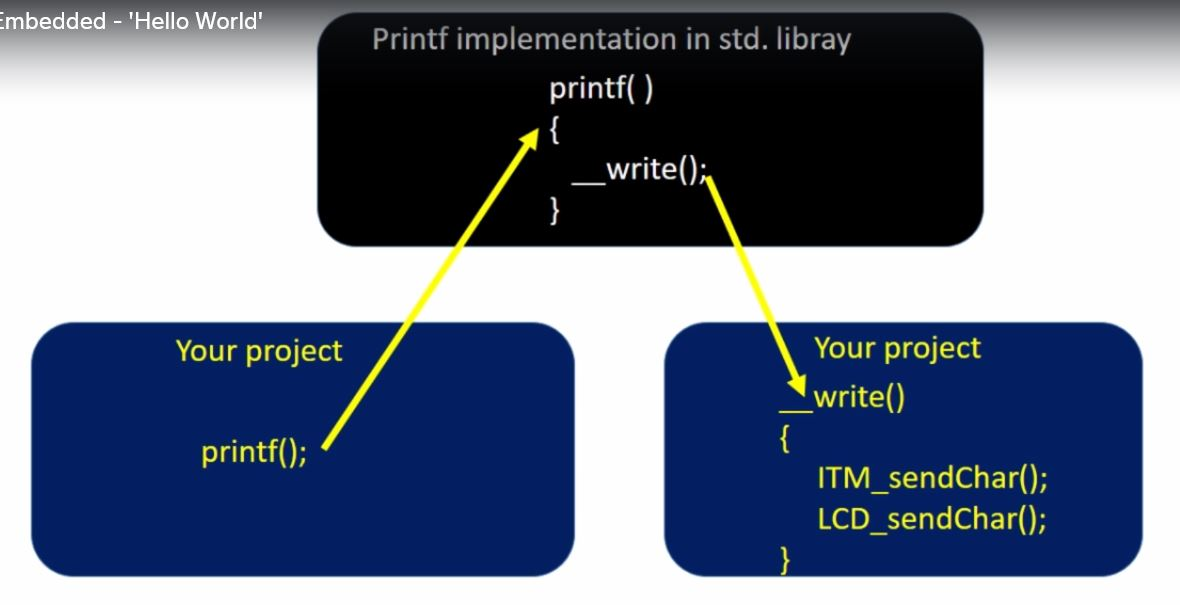
\includegraphics[scale=0.5]{Figures/Embedded_C/printf_debug_function_call}
\caption{Printf call function stack}
\label{fig:Embedded_C:printf_debug_function_call}
\end{figure} 

\subsection{Cross Compilation}

Now after saving the files of the source code, we need to build the project, and make what we call a \tbi{cross compilation}, as shown in \autoref{fig:Embedded_C:cross_compilation}.

\begin{figure}[h]
\centering
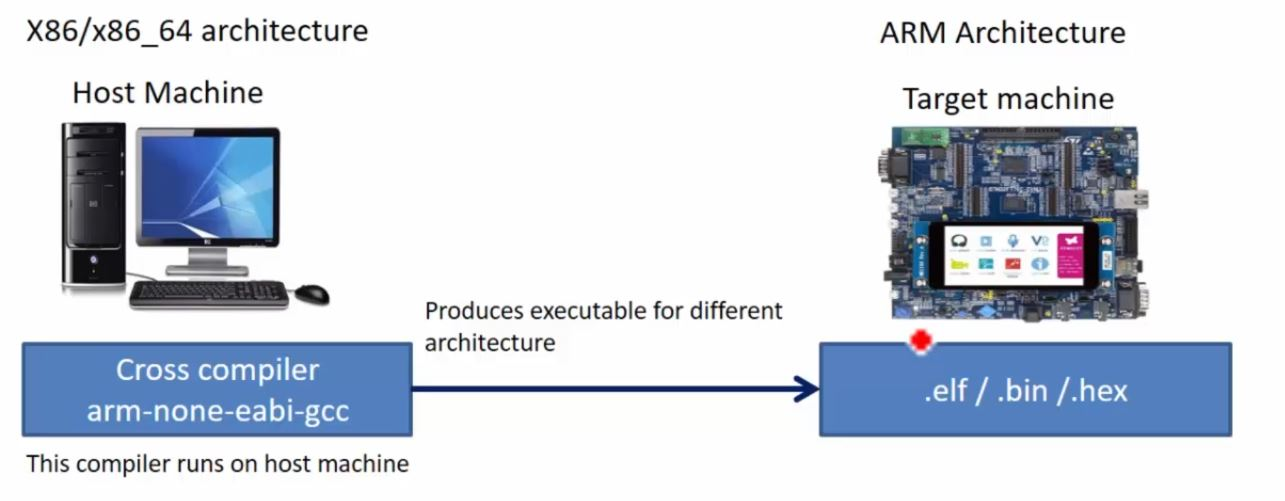
\includegraphics[scale=0.5]{Figures/Embedded_C/cross_compilation}
\caption{Cross Compilation: From host $\rightarrow$ to target stm32f40g}
\label{fig:Embedded_C:cross_compilation}
\end{figure} 

\begin{itemize}
    \item Cross compilation means that the executable code will be uploaded or done for a different architecture
    
    \begin{itemize}
        \item In our case, the cross compiler name is called arm-none-eabi-gcc, which is installed in the IDE and the toolchain
        
        \item Many type of executable format will be produced during the cross compilation:
        
        \begin{itemize}
            \item \verb|.elf|: executable for link format, used in debugging
            
            \item \verb|.bin| and \verb|.hex|, used for production
        \end{itemize}
        
        
    \end{itemize}
    
\end{itemize}


The opposite of cross compilation is \tbi{native compilation}, shown in \autoref{fig:Embedded_C:native_compilation}.

\begin{figure}[h]
\centering
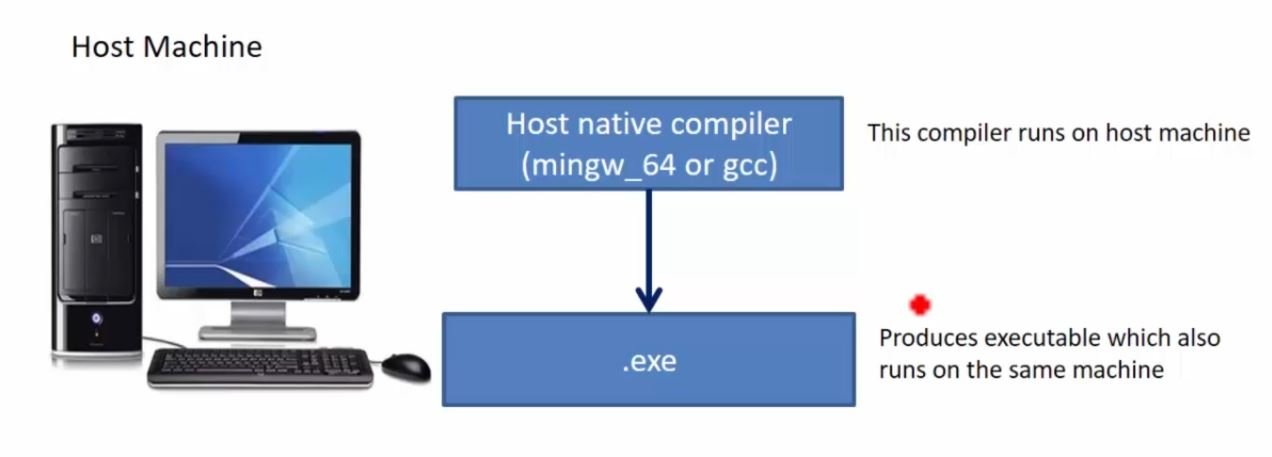
\includegraphics[scale=0.5]{Figures/Embedded_C/native_compilation}
\caption{Native compilation}
\label{fig:Embedded_C:native_compilation}
\end{figure} 


\subsection{Steps of building the project}
\label{SubSec:Steps_building_project}

The steps for printing hello world on stm32 board:

\begin{enumerate}

    \item Create a new project on the \tbi{target board} (review \autoref{Sub:Project on Board} to create a project)
    
    \item From github \url{https://github.com/niekiran/Embedded-C/blob/master/All_source_codes/target/stm32f407_disc/001HelloWorld/Src/syscalls.c}, add the snippet code about the implementation of \verb|void ITM_SendChar(uint8_t ch)|
    
    \begin{itemize}
        \item this function will send data to the board using ITM unit (see \autoref{Sub:Printing_hello_world})
    \end{itemize}
    
    \item Build the project 
    
    \item Now we need to load the project to the board.
    
    Connect the board to the pc
    
    \item Right click on the project, \verb|Debug As --> Debug Configuration|
    
    \item A pop window will appear , click on the left side \verb|STM32 MCU Debugging|, it will create a debug configuration
    
    \begin{itemize}
        \item On the tabs, click on \verb|Debugger|, then \verb|Debug probe| select the option \verb|ST-LINK GDB Server|
        
        \item In \verb|Interface|: it is \verb|SWD|
        
        \item In \verb|SWV|: we click for \verb|Enable| and we leave the clock options as it is
        
        \item Finally we close it
        
    \end{itemize}
    
    \newpage
    \item The right click on the project again, select \verb|Debug As --> STM32 MCU C/C++ Application|
    
    \begin{itemize}
        \item It will load the project on the board, and it will tell us to switch to debug perspective (we select \verb|ok|)
    \end{itemize}
    
    \item Now in order to see the \verb|printf|, we go to the \verb|Window Tab --> Show View --> SWV --> SWV ITM Console|
    
    \begin{enumerate}
        \item It will open the ITM console
        
        \item Click on the configure button (the tool logo), and select from \verb|ITM Stimulus port| port 0
        
        \item Click from the ITM console start trace (red circle) to accept data
        
        \item From the tab bar under \verb|Navigate|, click on \verb|run the code|
    \end{enumerate}
    
\end{enumerate}


\subsection{Back to Editing mode}

Once we finish up debugging, we need to go back to editing mode. This can be done using the button \verb|Teminate| (red square under \verb|Search Tab|)


\begin{itemize}
    \item \underline{Note:} In new version of stmcube IDE, there is \verb|terminate| button in the ITM console also, but it produces some bug and error, so don't use it and use the \verb|terminate| button under the \verb|Search| tab (see video 56 in section 8 to handle this error)
\end{itemize}


\subsection{Open OCD}

For older version of ARM cortex, we can use the Open OCD, which stand for \textit{open on chip debugger}.\\

See video 57 on section 8 later to write it (for now I won't use the open OCD since the SWD works).


\subsection{Some Extra Settings}

Let's see now how to explore data location and variable in memory.\\

Right click on the project name,select \verb|properties --> C/C++ Build --> Settings|, and it will open to us multiple option concerning the IDE and MCU.\\

\underline{Note:} there is nothing important for now, see video 60 in section 8 to hear their description, we will examine each of the feature and the settings later.

\newpage
\section{Build Process}

Now let's try to understand the build process. It is composed from various steps:

\begin{itemize}

\item Preprocessing

\item Parsing

\item Producing Object files

\item Linking object files

\item Producing final executable

\item Post processing on final executable

\end{itemize}


The above steps can be divided into 2 major steps: compilation and linking.\\

\underline{Compilation:}

\begin{figure}[h]
\centering
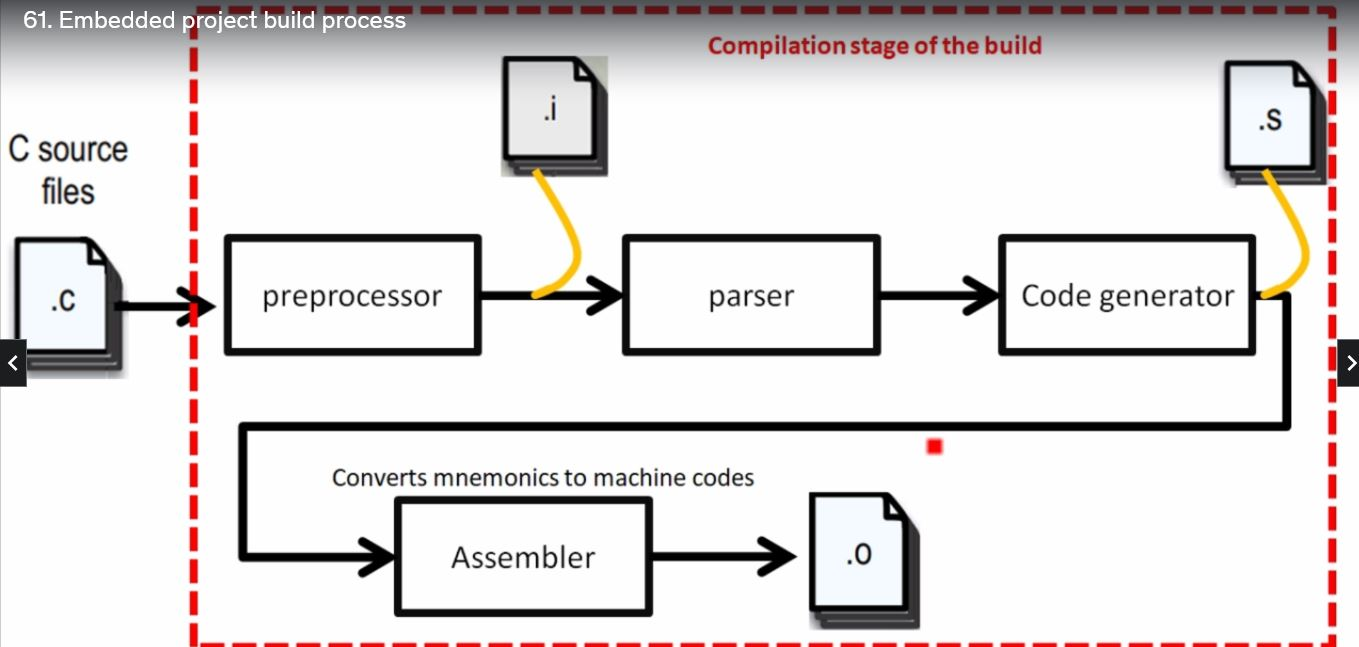
\includegraphics[scale=0.5]{Figures/Embedded_C/build_compiler_steps}
\caption{Compiler Steps}
\label{fig:Embedded_C:build_compiler_steps}
\end{figure} 

\begin{itemize}
    \item The preprocessor execute the \verb|#| statements
    
    \item Parser will ensure that syntax is correct
    
    \item Code generation: every C line code will turn into an assembly code
    
    \item Then the assembly code will turn to machine code \verb|.o|
    
    \begin{itemize}
        \item \underline{Note:} every C file will have its associated assembly file code \verb|.o|
    \end{itemize}
    
\end{itemize}

\newpage
Then it comes the linking stage.

\begin{figure}[h]
\centering
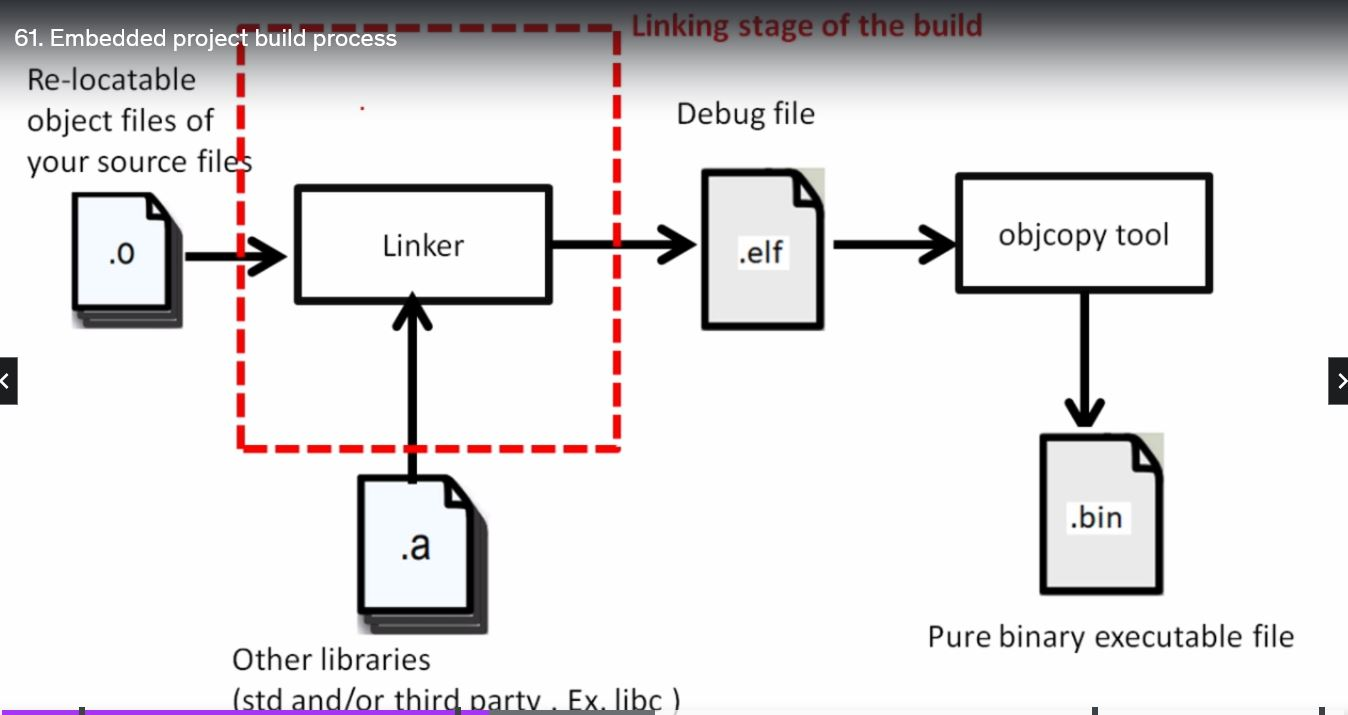
\includegraphics[scale=0.5]{Figures/Embedded_C/build_linker_steps}
\caption{Linker Steps}
\label{fig:Embedded_C:build_linker_steps}
\end{figure} 

\begin{itemize}
    \item All the \verb|.o| files will merge into 1 executable file: a \verb|.elf| file
    
    \item Then a postprocessing step using tools like objcopy will turn the \verb|.elf| to a 1 final binary file 
\end{itemize}

\newpage

\section{Analyzing C embedded Code}

Now we will take some C embedded code written for a MCU, and try to understand it. The list of points we try to uderstand are:

\begin{itemize}
    \item Anatomy of microcontroller
    
    \item Identifying code and data parts of the program
    
    \begin{itemize}
        \item Place of code in memory and data in memory
    \end{itemize}
    
    \item Disassembly feature using the IDE
    
    \item Analyzing the executable file \verb|.elf| using GNU tool such as objdump and size
    
\end{itemize}


\subsection{Anatomy of microcontroller}

A microcontroller is a small computer system on a ship, but with small resources compared to a desktop computer, because a microcontroller target embedded application.

In \autoref{fig:Embedded_C:anatomy_micro_1}, we have the different resources found on the ship of a microcontroller.

\begin{figure}[h]
\centering
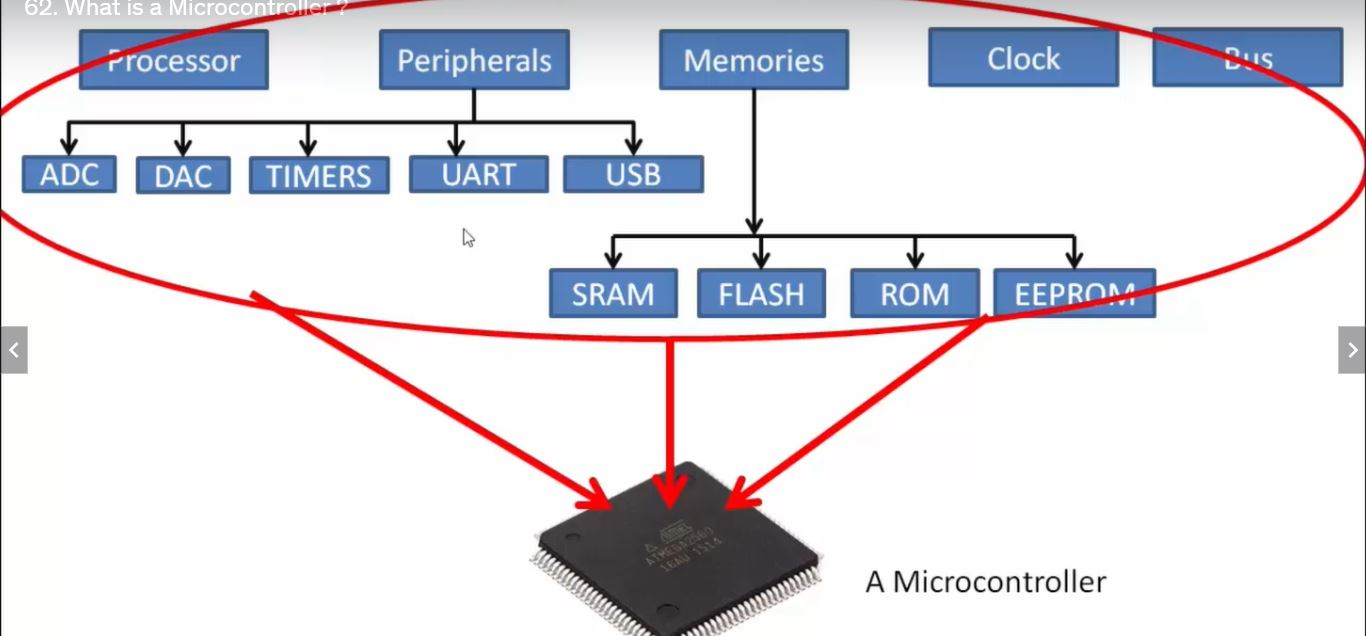
\includegraphics[scale=0.5]{Figures/Embedded_C/anatomy_micro_1}
\caption{Resources implemented inside a microcontroller ship}
\label{fig:Embedded_C:anatomy_micro_1}
\end{figure} 

\begin{itemize}
    \item In peripharls: some modules for \textit{connectivity} like UART and USB, for \textit{time} like TIMERS
    
    \item Memories: Volatile memory like SRAM, non-volatile like FLASH,ROM,EEPROM
\end{itemize}


\newpage
In \autoref{fig:Embedded_C:anatomy_micro_diagram}, we have a simple block diagram of a MCU.

\begin{figure}[h]
\centering
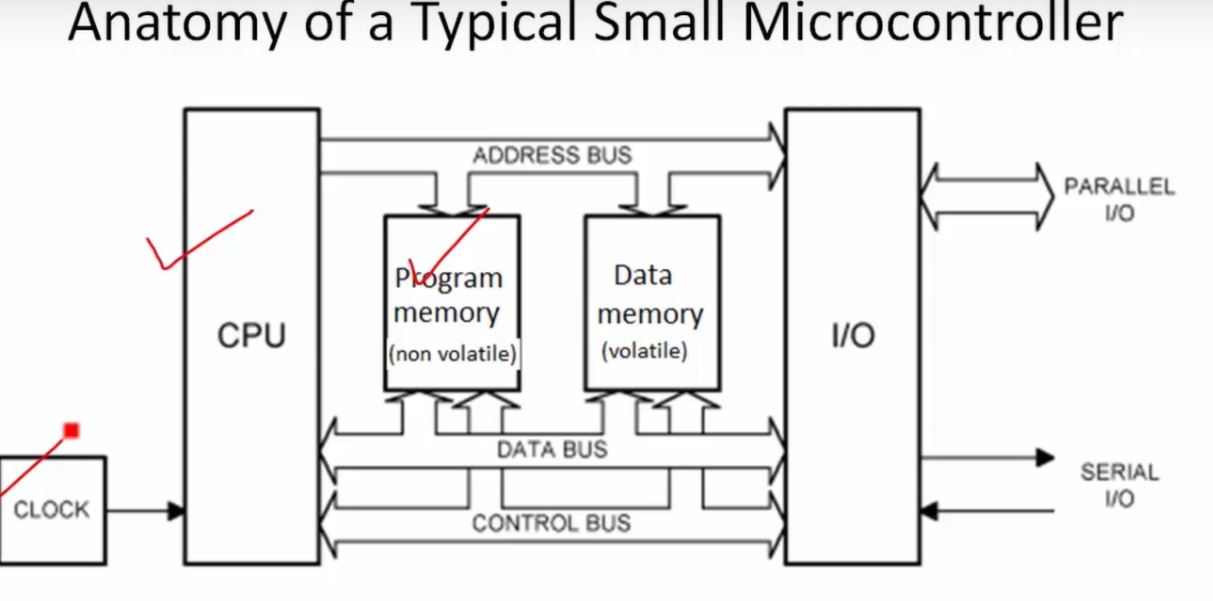
\includegraphics[scale=0.5]{Figures/Embedded_C/anatomy_micro_diagram}
\caption{Block diagram of MCU}
\label{fig:Embedded_C:anatomy_micro_diagram}
\end{figure} 

\begin{itemize}
    \item Every MCU contains a CPU (a processor) which produce instructions
    
    \begin{itemize}
        \item These instruction are stored inside the program memory (which are non-volatile)
        
        
        \item The speed of instruction handling depends on the clock
        
    \end{itemize}
    
    \item It contains I/O pins to communication with external world
    
\end{itemize}

Now we take some MCU used in industry.

\begin{itemize}
    \item STM32 
    
\begin{figure}[h]
\centering
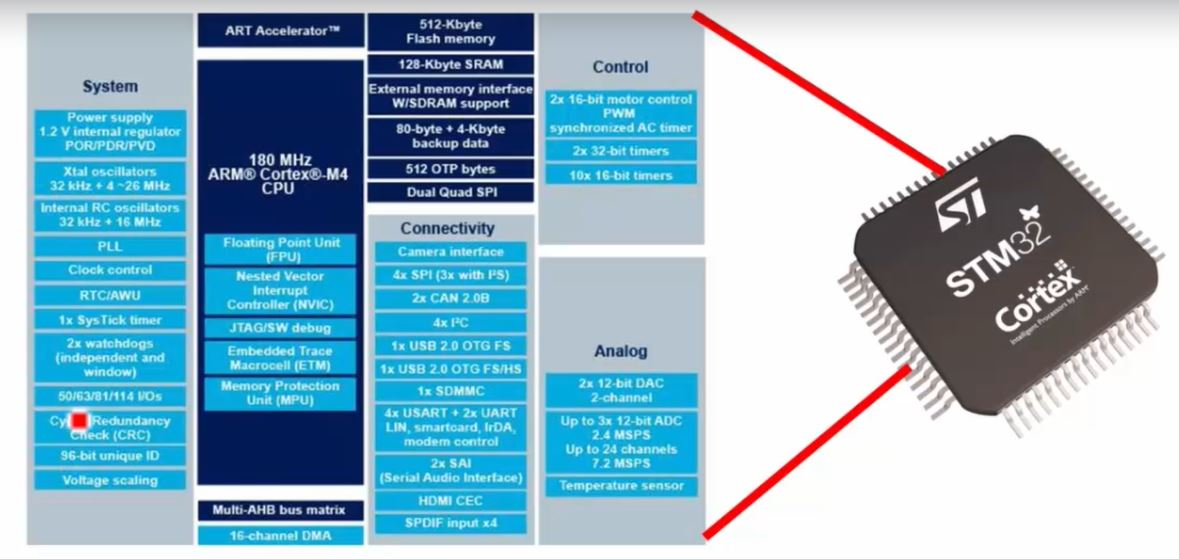
\includegraphics[scale=0.5]{Figures/Embedded_C/anatomy_micro_stm32}
\caption{Block diagram of MCU: STM32 MCU units}
\label{fig:Embedded_C:anatomy_micro_stm32}
\end{figure} 
    
The CPU of STM32 MCU are produced by arm company: it is an arm cortex CPU based, so it is not stm microelectronics who synthesised the CPU    
    
\end{itemize}


\subsection{Code Memory}

Code memory is where we store our code and constant data, and the memory type is non-volatile.\\

There are many type of code memory circuity, like ROM (alos ROM have different types such as EEPROM,MPROM,$\cdots$), FLASH (which is used in stm32 MCU units, and they are very cheap).\\

Another type of memory is  , which is very fast in access time, thus making the price of microncontroller to shoot up.

In stm32 reference manual, chapter 3, the FLASH is of size 512 KB, and it is also divided into several sectors/block.


\subsection{Tracking variable in the memory}

Refer to the \verb|main| of the project named \verb|Tracking-variables-memory|.

\begin{enumerate}
    \item Once we finish writing the code, we need to \tbi{build the project} in order to have at the end the \verb|.elf| file
    
    
    \item To load the code to the microncontroller, we need to 
    
    \verb|Debug as --> STM32 MCU C/C++ Application|
    
    \begin{itemize}
    
    
    \item Review setting of \ref{SubSec:Steps_building_project}.
    
    
        \item A console log window will appear and tell us that \verb|Download verified successfully |
        
        More specifically, the data will go to the \verb|FLASH|
        
    \end{itemize}
    

    \newpage
    \item First, we need what is called \tbi{the base address} of the \verb|FLASH| memory.
    
    We go to the reference manual, Table 5 in section 3.3, shown in \autoref{fig:Embedded_C:falsh_memory_Table}.
    
    
    \begin{figure}[h]
\centering
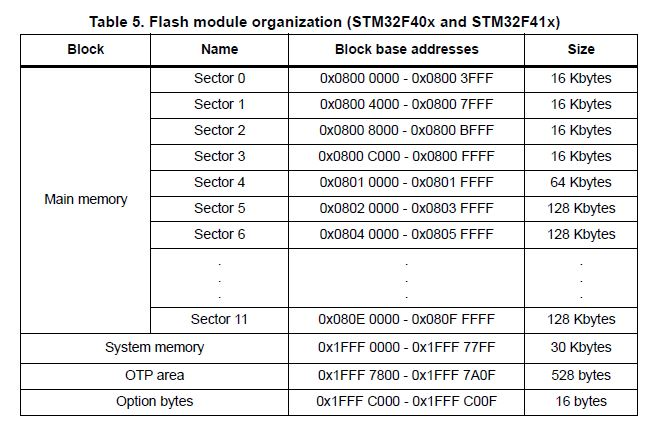
\includegraphics[scale=0.5]{Figures/Embedded_C/falsh_memory_Table}
\caption{Flash Memory organization}
\label{fig:Embedded_C:falsh_memory_Table}
\end{figure} 
    
    
    \begin{itemize}
        \item It is a total of 512 KByte memory
        
        \item It is a read only memory, also we call it \tbi{system memory}
        
    \end{itemize}
    
The base address start from the $\mathrm{1}^\mathrm{st}$ line  \verb|0x0800 0000|, and we can use the memory till sector 11, of final address is \verb|0x080F FFFF|


\item To see the content of the \verb|FLASH| (or any other type of memory), we go to \verb|Window --> Memory| or \verb|Memory content|, then type the base address \verb|0x0800 0000|.

\item Now the \verb|FLASH| is for the program code. 

For the data code, we need the address of \verb|SRAM|

\begin{itemize}
    \item In stm32 we have 2 \verb|SRAM|: \verb|SRAM1| the main one, and \verb|SRAM2| an auxiliary one
    
    \item There addresses can be found in chapter 2 in the reference \todo{SRAM} \textit{to search for it later}
\end{itemize}
    
    
    
\end{enumerate}


\underline{Note:} the data get transferred from \verb|FLASH --> SRAM| by routines and handler written in assembly in the \verb|Startup| folder of the project.

See video 65 for more details to navigate through the content (but it is not important for now).

\newpage
\subsection{Disassembly}

Now we will see how to disassembler work in the IDE. First we need to go into debug mode, by \verb|Debug --> Stm32 C/C++ Application|, then we go to \verb|Window --> Show View --> Disassembly|.\\

It will open to us an disassembly window, showing us the assembly code of our program.

The goal of such debugging is if we want to optimize at a instruction level, or understand what is happening at the assembly level.\\

We can do 2 types of debugging:

\begin{enumerate}
    \item C code debugging: by inserting break points
    
    \item Assembly code: by inserting break points in the disassembly window or by enable instruction mode (the i logo with $\rightarrow$ under the \verb|Run tab|)
\end{enumerate}

Review video 66 and 67 from section 10 for more details. 

\newpage
\section{Floating Point numbers}

Now we move to how real numbers are stored in the memory.

In computers, real numbers (with comma) are stored according to IEEE75 floating point system.\\

\underline{Goal of floating system:} in case we are working with very small (charge of electron) or very big (distance between earth and sun), we can't use type \verb|long long| for example, that's why we use floating point number.

\subsection{IEEE75 floating}

Suppose for example we have to store $+ 7.432 \times 10^{48}$. We can't store its binary equivalent because it will consume allot of memory.

Instead, we store the important part as shown in \autoref{fig:Embedded_C:ieee75_example_1}


\begin{figure}[h]
\centering
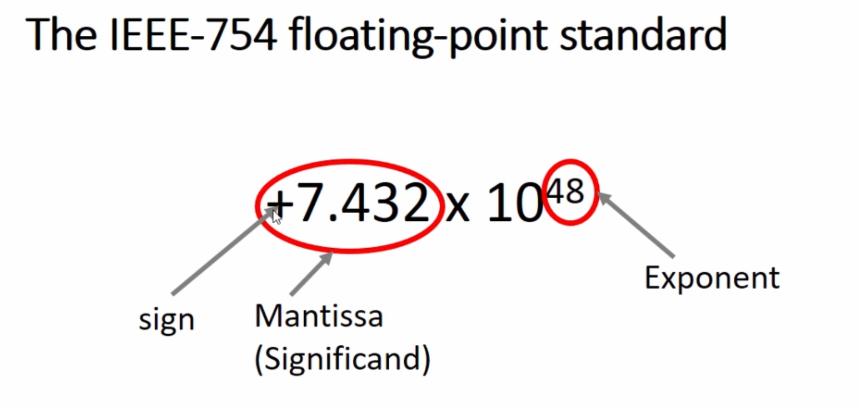
\includegraphics[scale=0.5]{Figures/Embedded_C/ieee75_example_1}
\caption{Floating Point Example}
\label{fig:Embedded_C:ieee75_example_1}
\end{figure} 

By this way, we will \textit{approximate} the number and store only the important part in the memory, which are the essential components to give the value of the number.\\

\underline{How we store:}

There are 2 ways to store the main part of \autoref{fig:Embedded_C:ieee75_example_1}:

\begin{enumerate}
    \item Single precision shown in \autoref{fig:Embedded_C:ieee75_single_precision}. 
    
\begin{figure}[h]
\centering
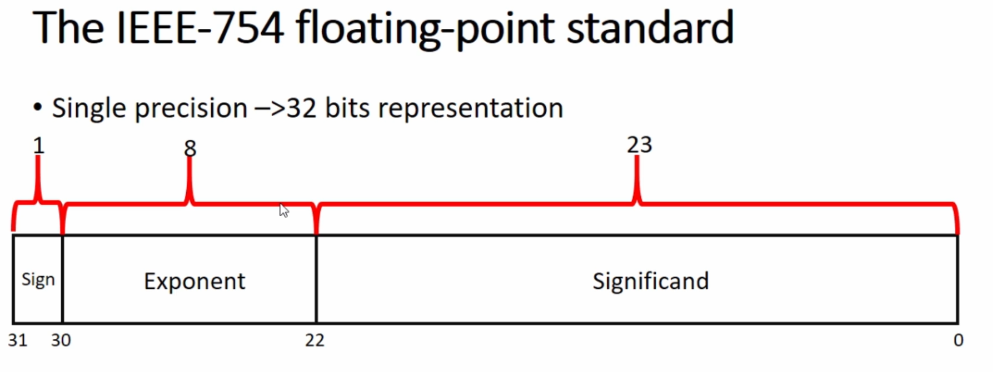
\includegraphics[scale=0.5]{Figures/Embedded_C/ieee75_single_precision}
\caption{IEEE-745 Single Precision}
\label{fig:Embedded_C:ieee75_single_precision}
\end{figure} 

For float: storage is 4 bytes, precision up to 6 decimal places, and range from  $1.2 \times 10^{-38} \rightarrow 3.4 \times 10^{38}$
    
\newpage    
    \item Double precision (more accurate but consume more memory) shown in \autoref{fig:Embedded_C:ieee75_double_precision}.
    
\begin{figure}[h]
\centering
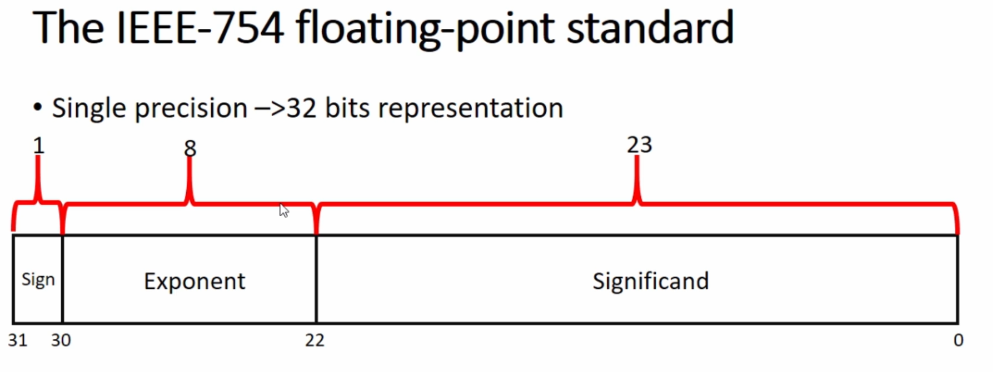
\includegraphics[scale=0.5]{Figures/Embedded_C/ieee75_single_precision}
\caption{IEEE-745 Double Precision}
\label{fig:Embedded_C:ieee75_double_precision}
\end{figure}

For double: storage is 8 bytes, precision up to 15 decimal places, and range from  $2.3 \times 10^{-308} \rightarrow 1.7 \times 10^{308}$
    
\end{enumerate}


\underline{Format Specifier:} \verb|%lf| for double and \verb|%f| for float.

An example for handling floating point using charge of electron is shown in \autoref{fig:Embedded_C:ieee75_example_code}.

\begin{figure}[h]
\centering
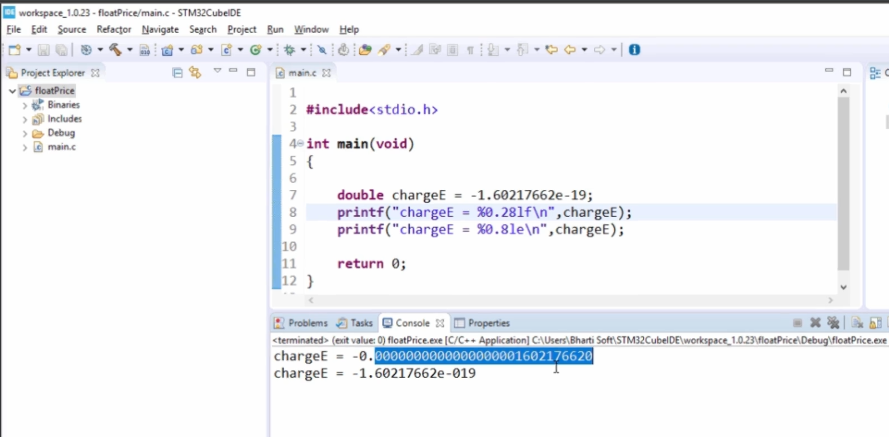
\includegraphics[scale=0.5]{Figures/Embedded_C/ieee75_example_code}
\caption{Example Code for floating point}
\label{fig:Embedded_C:ieee75_example_code}
\end{figure} 


Some nice thing for small number is the formatting using scientific notation, using the format specifier \verb|e|


\newpage

\section{Scanf}

When using \verb|scanf|, in some console it causes the console to store in the output buffer. In other words, the output stream get stucked because we are waiting for user command.

This is because when using the \verb|printf| function, the stream doesn't go directly to the console, but it goes to some output buffer, where we have a buffer API which output the stream to the console, as shown in \autoref{fig:Embedded_C:printf_buffer}.


\begin{figure}[h]
\centering
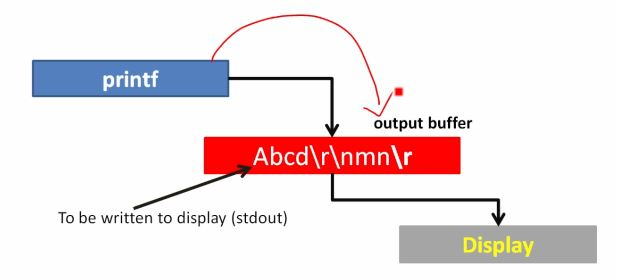
\includegraphics[scale=0.5]{Figures/Embedded_C/printf_buffer}
\caption{Flash Memory organization}
\label{fig:Embedded_C:printf_buffer}
\end{figure} 


In order to output the stream from the output buffer to the screen, we use the function \verb|fflush(stdout)|.

\underline{Note:} video 72 contain nice explanation about input buffer for storing strings. To understand it later.


\newpage
\section{Pointers}

Pointers are used in embedded programming in order to access peripheral, read/write data to them.\\

To recap, pointers are just addresses of variables, as shown in \autoref{fig:Embedded_C:pointer_recap}.


\begin{figure}[h]
\centering
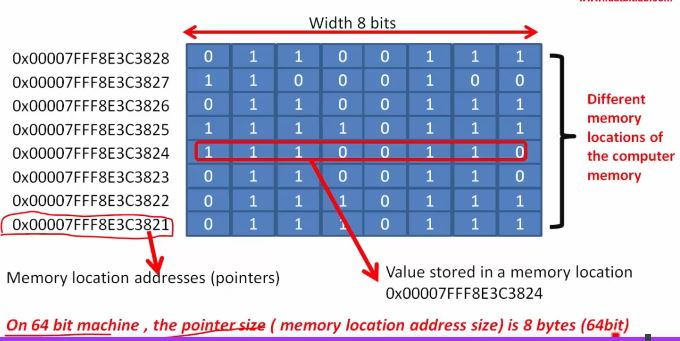
\includegraphics[scale=0.5]{Figures/Embedded_C/pointer_recap}
\caption{Pointers}
\label{fig:Embedded_C:pointer_recap}
\end{figure} 

\underline{Operations:} we can decrement a pointer to reach memory addressee beneath current location (or increment, to go up in memory), and we can access the data in memory via the pointer.\\

\underline{Steps:}

\begin{enumerate}
    \item Initialize the data \verb|int data = 5|
    
    \item Pointer assignment to data \verb|int* p_data = &data|
    
    \begin{itemize}
        \item The pointer data type is the same as data type (pointer pf type int, so the data is of type int)
    \end{itemize}
    
    \item Access the content via the pointer \verb|value = *p_data|, where \verb|*| is the dereferencing operator
    
\end{enumerate}

Important notes about pointers:

\begin{itemize}
    \item Whatever the data type, the pointer content (addresses) have 8 byte
    
    \begin{itemize}
        \item This means that \verb|int*| and \verb|char*| will have 8 bytes addresses
    \end{itemize}
    
    \item But the value will be different
    
    \begin{itemize}
        \item \verb|int* p_data = &data|, \verb|*p_data| will have 4 bytes because we have \verb|int| data type
        
        \item \verb|char* p_data_2 = &data_2|, \verb|*p_data_2| will have 1 byte because we have \verb|char| data type
    \end{itemize}
    
    
\end{itemize}

\todo{Pointer Arithmetic}: \textit{To redo video 63 on pointer arithmetic}

\underline{Take away:} when incrementing pointer by 1, we move by the size of the data type.\\

Example: if we have \verb|int* p_data|, that is a pointer to \verb|int|, the +1 will be an offset of 4 byte because size of int is of 4 bytes.

\newpage

\section{stdint and Portability}

Suppose we wrote come C code, and we are testing our program with 2 compilers (because we are using 2 hardware for example, smt32 and PIC for example). Each of the hardware have its own compiler. Although the C code is correct, our code may have some buggy issues due to compiler design, that is each designer will design different byte size for data type according to the specific hardware architecture, which differ from hardware to hardware.\\

For example, for MPLAB compiler (for the PIC microcontroller), the \verb|int| data type has 2 byte allocation (shown in \autoref{fig:Embedded_C:data_type_IDE}), whereas the in stm IDE the int data type has 4 byte allocation.


\begin{figure}[h]
\centering
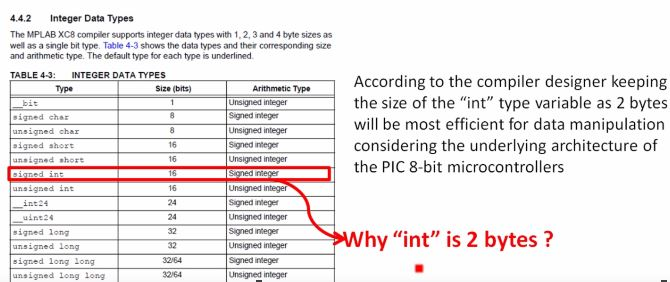
\includegraphics[scale=0.5]{Figures/Embedded_C/data_type_IDE}
\caption{Data Allocation}
\label{fig:Embedded_C:data_type_IDE}
\end{figure} 

The reason is also behind this freedom is that C standard have given the freedom to compiler designer to choose based on optimum hardware design for data type \verb|int| and \verb|long|

Take an example the code shown in \autoref{fig:Embedded_C:code_portability_1}.

\begin{figure}[h]
\centering
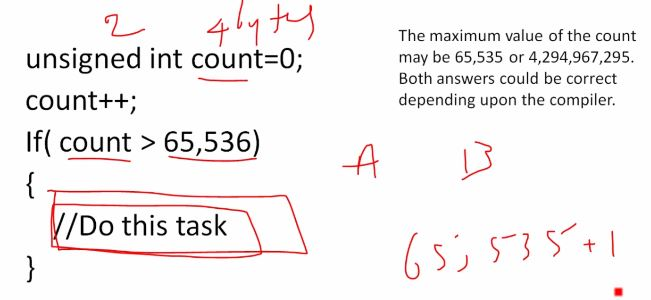
\includegraphics[scale=0.5]{Figures/Embedded_C/code_portability_1}
\caption{Code portability}
\label{fig:Embedded_C:code_portability_1}
\end{figure} 

If \verb|unsigned int| have 2 bytes, then the max is $2^{16} -1 = 65 535$, and when reaching 65 535 +1, the \verb|while| loop won't enter and the code won't work anymore.\\

\newpage
To avoid such problems, we will instead of true variable data type, their aliases in the \verb|stdint.h| file, as shown in \autoref{fig:Embedded_C:aliases_data_type}.


\begin{figure}[h]
\centering
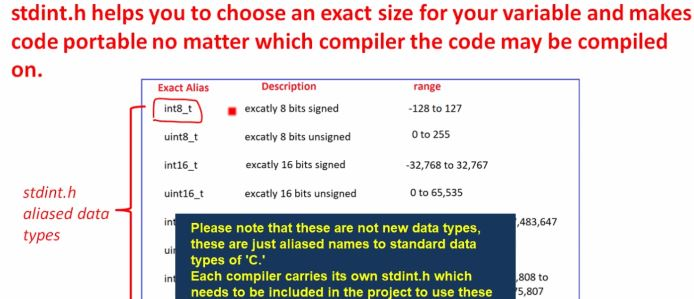
\includegraphics[scale=0.5]{Figures/Embedded_C/aliases_data_type}
\caption{Code portability}
\label{fig:Embedded_C:aliases_data_type}
\end{figure} 


Some of useful aliases data type which we will use in programming are shown in \autoref{fig:Embedded_C:aliases_data_type_useful}

\begin{figure}[h]
\centering
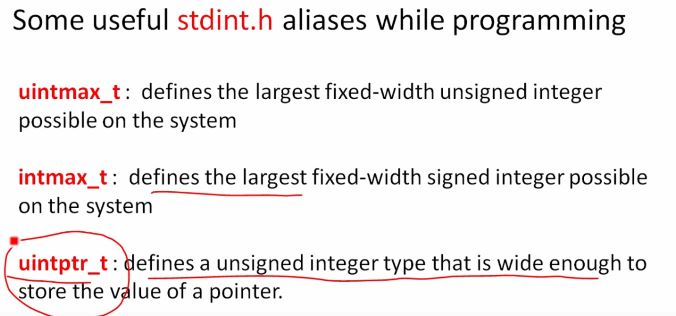
\includegraphics[scale=0.5]{Figures/Embedded_C/aliases_data_type_useful}
\caption{Code portability}
\label{fig:Embedded_C:aliases_data_type_useful}
\end{figure} 

\newpage
\section{Bitwise Operation}

Bitwise operation plays an important role in embedded programming, accessing registers,$\cdots$. They are built up upon our understanding of number systems and logic gates.\\

First a recap about logic gates:


\begin{table}[!h]
\centering
\begin{tabular}{c| c }
Symbol 	& Description\\ \hline
$|$	& OR gate: 1 if any operand contains 1  \\ \hline
\verb|&|	& AND gate: 1 if the 2 operand contains 1 at the same time  \\ \hline
\verb|^| & XOR: 1 if 1 of the operand contains 1, but not both (we exclude this case) \\ \hline
\verb|~|& NOT operation \\ \hline
\verb|<<| & left shift operator: left shift by some number of bits \\ \hline
\verb|>>| & right shift operator: left shift by some number of bits \\ \hline

\end{tabular}
\caption{Bitwise Operation used in embedded programming}
\label{Tb:Bitwise_Operation:reminder}
\end{table}

\underline{Note:} the \verb|>>| and \verb|<<| are important because they enable us to set bits in registers without affecting the other bit positions. The other bits maybe connected to other things or we don't know what they do.\\

Another point, that in C language, we have also logical AND (\verb|&&|), logical OR ($||$), and logical NOT (!). 

The difference between them and operator in \autoref{Tb:Bitwise_Operation:reminder}, is that these operator act directly on non binary level, whereas bitwise are in bit level (example for OR is shown in \autoref{fig:Embedded_C:bitwise_logical_OR}).

\begin{figure}[h]
\centering
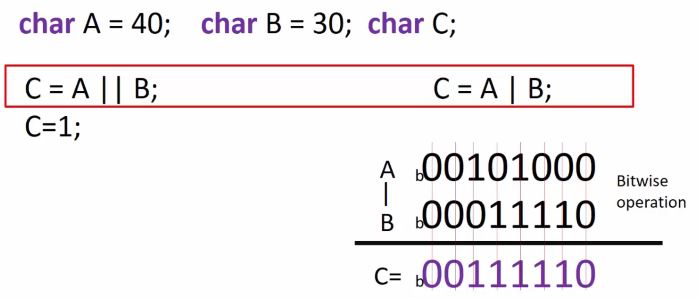
\includegraphics[scale=0.5]{Figures/Embedded_C/bitwise_logical_OR}
\caption{Difference between logical OR and bitwise OR}
\label{fig:Embedded_C:bitwise_logical_OR}
\end{figure} 

Usually we have 4 operations in embedded programming:

\begin{enumerate}
    \item Testing bit (\verb|&|)
    
    \item Setting of bits ($|$)
    
    \item Clearing of bits (\verb|~|, \verb|&|)
    
    \item Toggling of bits (\verb|^|)
    
\end{enumerate}



\newpage
\subsection{Testing bit}

Suppose we have some number, and we want to test some bits in some position $x$. An example is shown in \autoref{fig:Embedded_C:testing_bit}.

\begin{figure}[h]
\centering
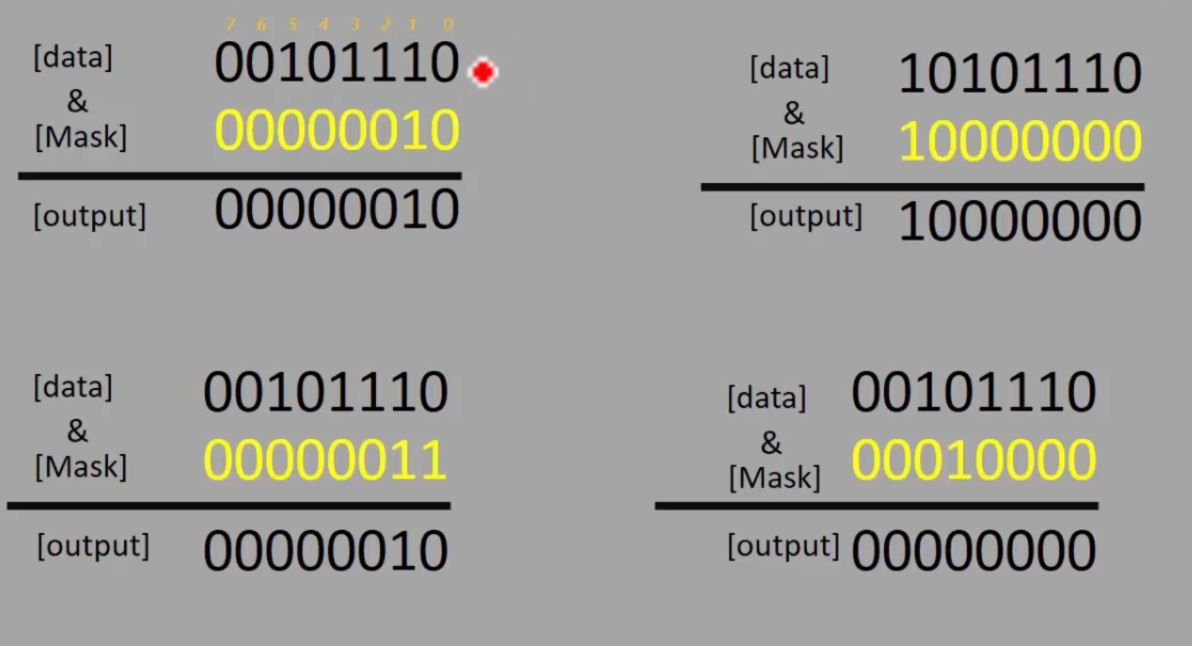
\includegraphics[scale=0.5]{Figures/Embedded_C/testing_bit}
\caption{Testing bit using and operation and masking}
\label{fig:Embedded_C:testing_bit}
\end{figure} 

\begin{itemize}
    \item In the $\mathrm{1}^\mathrm{st}$ example, we want to test bit in position 1, so we set the mask in this position to 1 and all other 0
    
    \item This is because $x$ \verb|&| 1 = $x$, so we know the identity of $x$, and for other bit position we don't care, we set the mask to 0
\end{itemize}


\newpage
\subsection{OR}

Now we will take some 8 bit register example, and we to say that we want to set 1 in the $\mathrm{1}^\mathrm{st}$ bit field of this register.\\

The syntax for doing so: \verb|PortB| $|$ \verb|mask|. An example is shown in \autoref{fig:Embedded_C:setting_bit}. 

\begin{figure}[h]
\centering
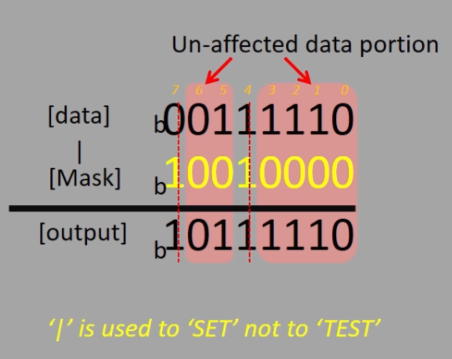
\includegraphics[scale=0.7]{Figures/Embedded_C/setting_bit}
\caption{Setting bits using OR}
\label{fig:Embedded_C:setting_bit}
\end{figure} 



\underline{OR masking to remember:} The key thing about OR masking is that the mask 1 column will give us 1 no matter the content in the port, and the remaining will be unchanged.

So the OR is a good operation to set some bits to 1 and keep the rest unchanged.

\subsection{XOR}

The XOR operation can be served a flipping, same as the OR: it flipping the bit in the column mask, and the other remains unchanged. An example is shown in \autoref{fig:Embedded_C:toggling_xor}.

\begin{figure}[h]
\centering
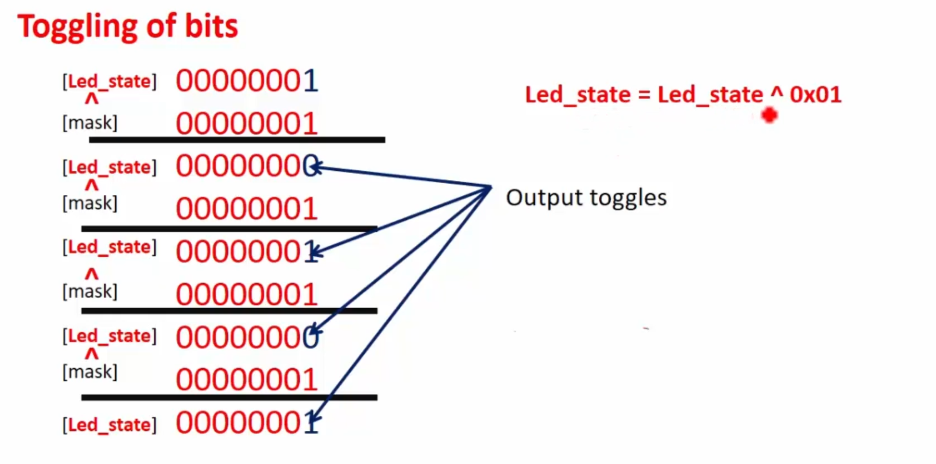
\includegraphics[scale=0.5]{Figures/Embedded_C/toggling_xor}
\caption{LED Toggling with XOR}
\label{fig:Embedded_C:toggling_xor}
\end{figure}

\newpage
\section{LED Practice}
\label{Sec:Led_practice}

Now we will use bitwise operation, pointers in order to turn on LED on our board. 


\subsection{Hardware GPIO,Bus}
\label{Sub:Hardware_GPIO_Bus}

First, we need to understand hardware connection to our board. For this purpose, we download the \textit{schematic board} for the STM40 discovery board form stm website, in resource section.\\

\autoref{fig:Embedded_C:LED_connection} shows the LED in our SMT32F40 discovery board.
 
 
\begin{figure}[h]
\centering
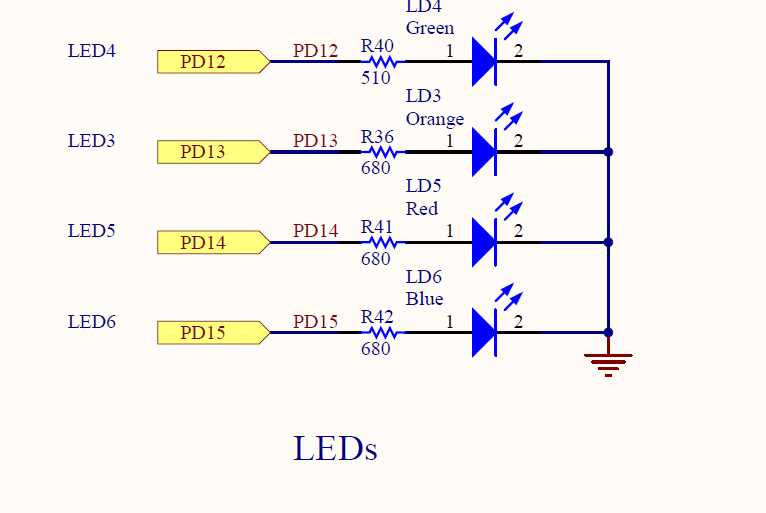
\includegraphics[scale=0.7]{Figures/Embedded_C/LED_connection}
\caption{LED Connection to SMT32F40 discovery board}
\label{fig:Embedded_C:LED_connection}
\end{figure}

\begin{itemize}
    \item \verb|PD15| stands for port D, pin 15.
\end{itemize}

\newpage
\tbi{In the schematic} also, we \tbi{can find the ports in the board}, shown in  \autoref{fig:Embedded_C:ports}

\begin{figure}[h]
\centering
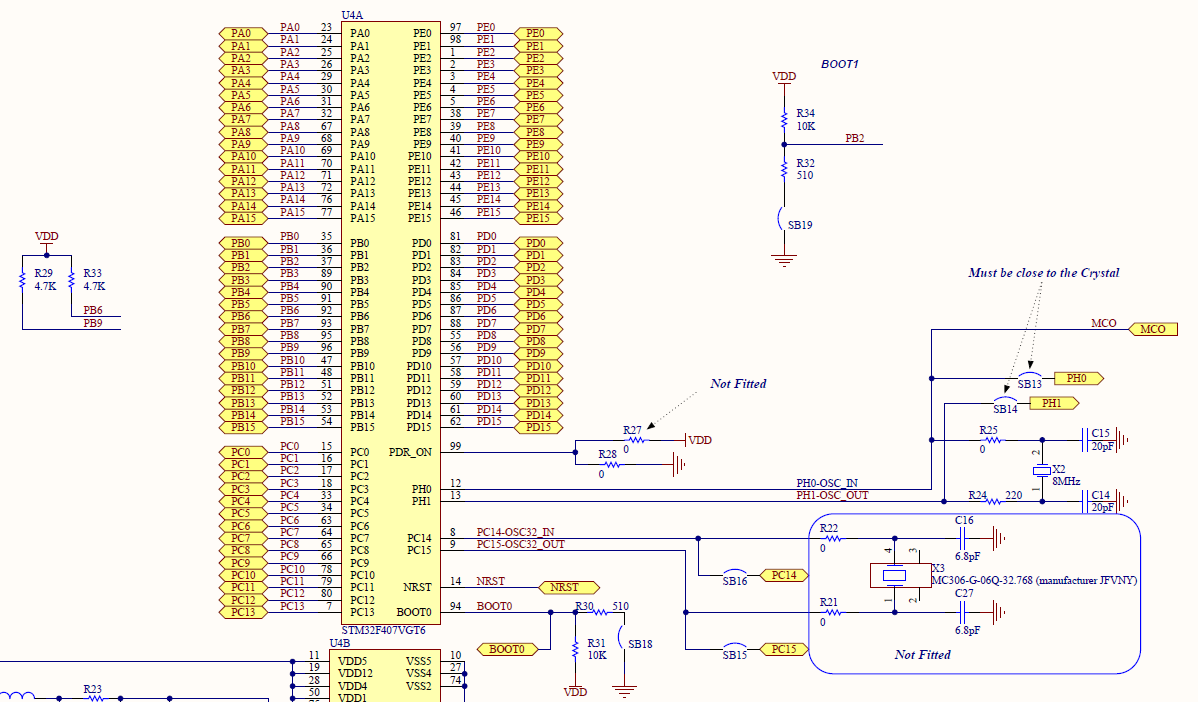
\includegraphics[scale=0.7]{Figures/Embedded_C/ports}
\caption{Ports of SMT32F40 discovery board}
\label{fig:Embedded_C:ports}
\end{figure}

\begin{itemize}
    \item In stm32Fx series, each port has 16 pins
    
    \item We can connect to them external peripheral (LED,display,button, Bluetooth transceiver,external memory,$\cdots$)
\end{itemize}

\newpage
Now back to \autoref{fig:Embedded_C:LED_connection}. Suppose we want to access the green LED, so we need to control \verb|PD12|.


How we can do so? \autoref{fig:Embedded_C:gpio_d_software} contains the answer.
 
\begin{figure}[h]
\centering
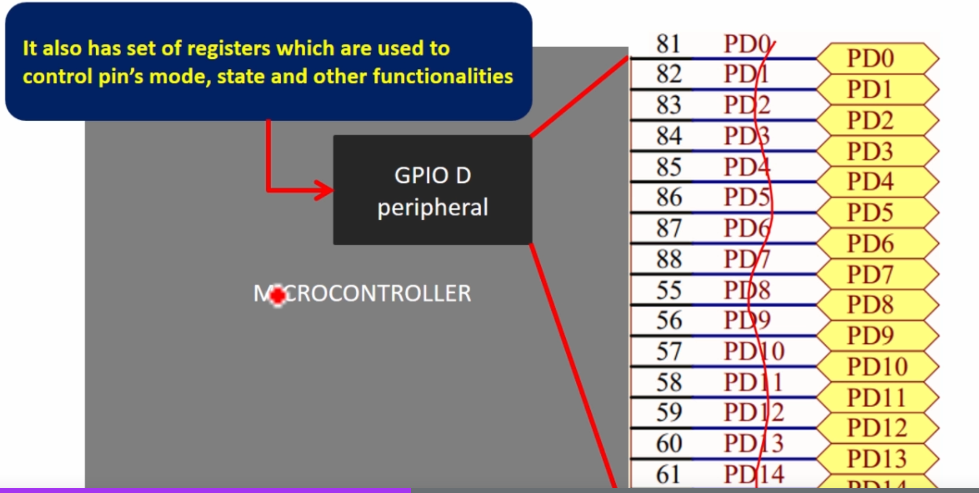
\includegraphics[scale=0.7]{Figures/Embedded_C/gpio_d_software}
\caption{Controlling port D from GPIO D peripheral}
\label{fig:Embedded_C:gpio_d_software}
\end{figure}
 
Port D is controlled via a \textit{peripheral} called GPIO D, which contains a register controlling the port D (mode of each pin,state,function,$\cdots$).\\

\tbi{Each register} in GPIO D \tbi{contains its own address}, and if we want to use some register, we need to access via its unique address via the data bus as shown in \autoref{fig:Embedded_C:data_bus_connecting_peripheral}.

\begin{figure}[h]
\centering
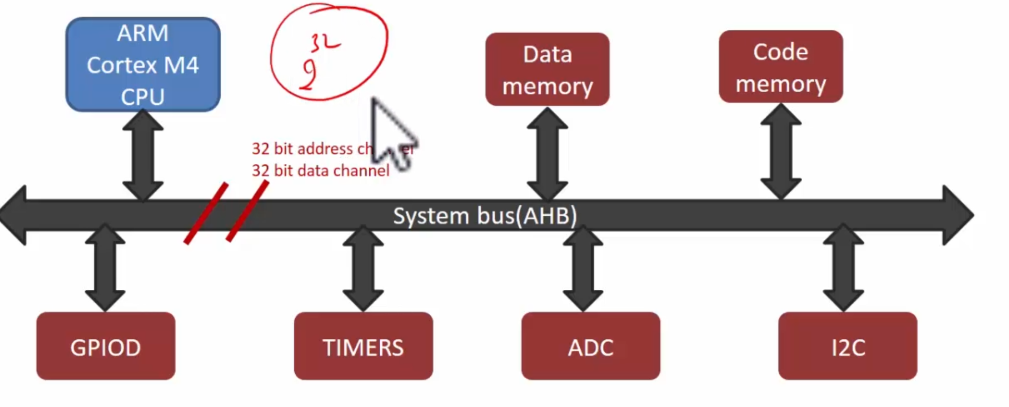
\includegraphics[scale=0.7]{Figures/Embedded_C/data_bus_connecting_peripheral}
\caption{Data bus Connecting peripheral}
\label{fig:Embedded_C:data_bus_connecting_peripheral}
\end{figure}

\begin{itemize}
    \item AHB stand for advanced High-performance Bus, created by st
    
    \item The width of the bus is 32 bits, which means we can put $2^{32}$ addresses as shown in \autoref{fig:Embedded_C:data_bus_width}.
\end{itemize}

\begin{figure}[h]
\centering
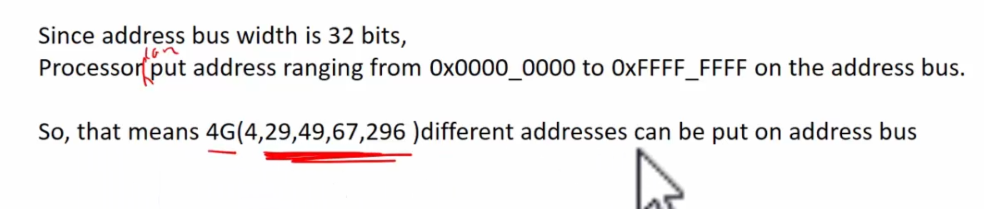
\includegraphics[scale=0.7]{Figures/Embedded_C/data_bus_width}
\caption{Data bus width and addresses range}
\label{fig:Embedded_C:data_bus_width}
\end{figure}

\newpage
The memory map of ARM cortex Mx processor is shown in \autoref{fig:Embedded_C:memory_map}.

\begin{figure}[h]
\centering
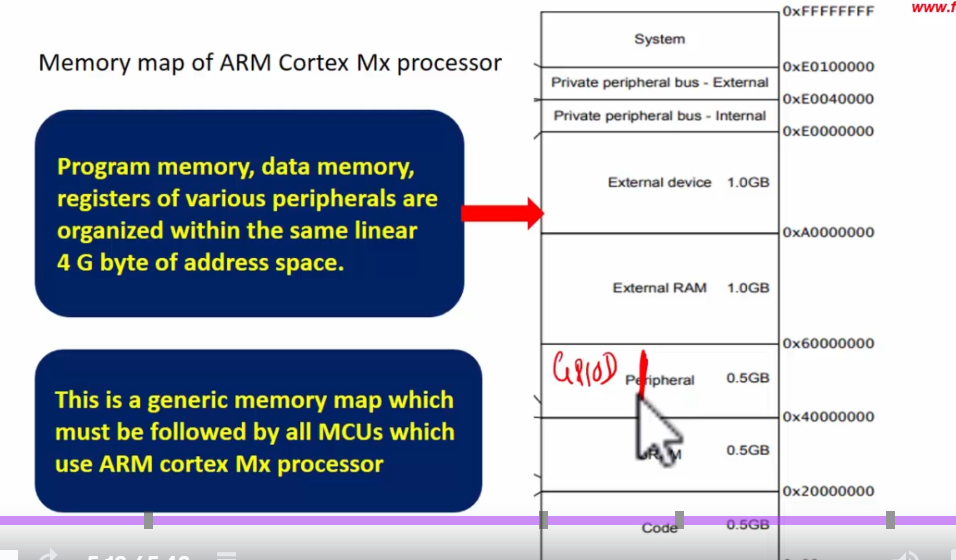
\includegraphics[scale=0.7]{Figures/Embedded_C/memory_map}
\caption{Memory Map}
\label{fig:Embedded_C:memory_map}
\end{figure}

To know what is GPIO D address (or any other peripheral we want to access it), we go to the reference manual, section 2.3 (Memory map), Table 1, and we find for GPIO D \verb|0x 4002 0C00| as base address (starting address) for GPIO D.

\newpage
\subsection{Peripheral Information}
\label{Sub:Peripheral_Information}

\begin{itemize}
    \item All stm32 peripheral are 32 bit wide
    
    \item Different peripheral have different number of registers (GPIO D may have 10 register, and ADC may have 8 register)
    
    \item An example about GPIO D registers are shown in \autoref{fig:Embedded_C:gpio_d_registers}.
    
\begin{figure}[h]
\centering
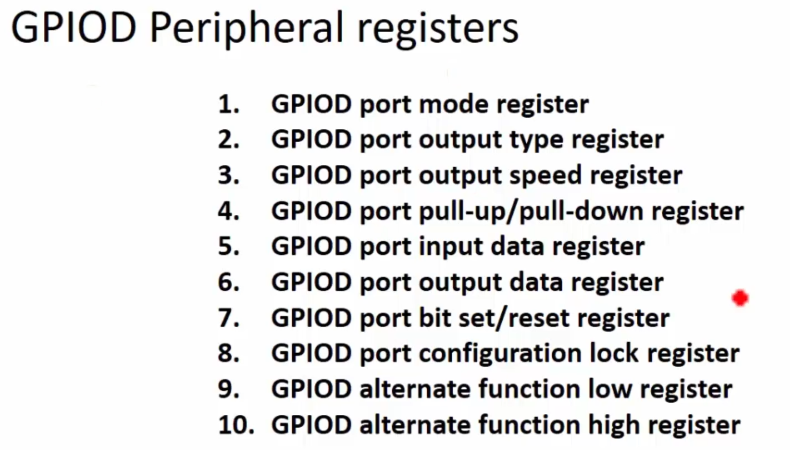
\includegraphics[scale=0.7]{Figures/Embedded_C/gpio_d_registers}
\caption{Different peripheral registers for GPIOD}
\label{fig:Embedded_C:gpio_d_registers}
\end{figure}    
    
Each of the 10 register is of 32 bit width, and has its own start and end addresses as shown in \autoref{fig:Embedded_C:gpio_d_registers_addresses}

\begin{figure}[h]
\centering
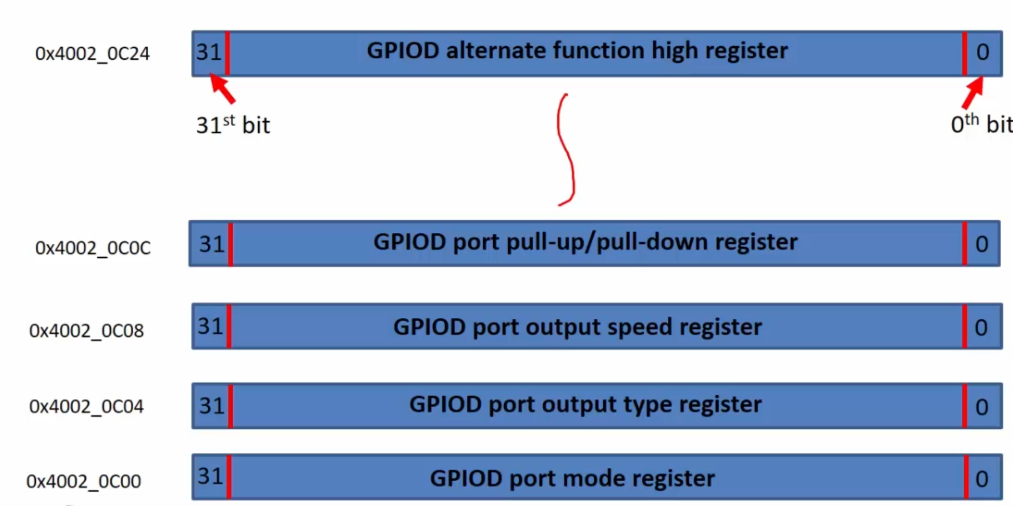
\includegraphics[scale=0.7]{Figures/Embedded_C/gpio_d_registers_addresses}
\caption{GPIOD Register Addresses}
\label{fig:Embedded_C:gpio_d_registers_addresses}
\end{figure}  

Each of these register has its own purpose, like GPIO mode register is used to configure the port pins as output or input. Also an example is shown in \autoref{fig:Embedded_C:gpio_d_data_registers}, where the data register is used to turn on LED ON or OFF (by setting bits 0 for OFF or 1 for ON)

\begin{figure}[h]
\centering
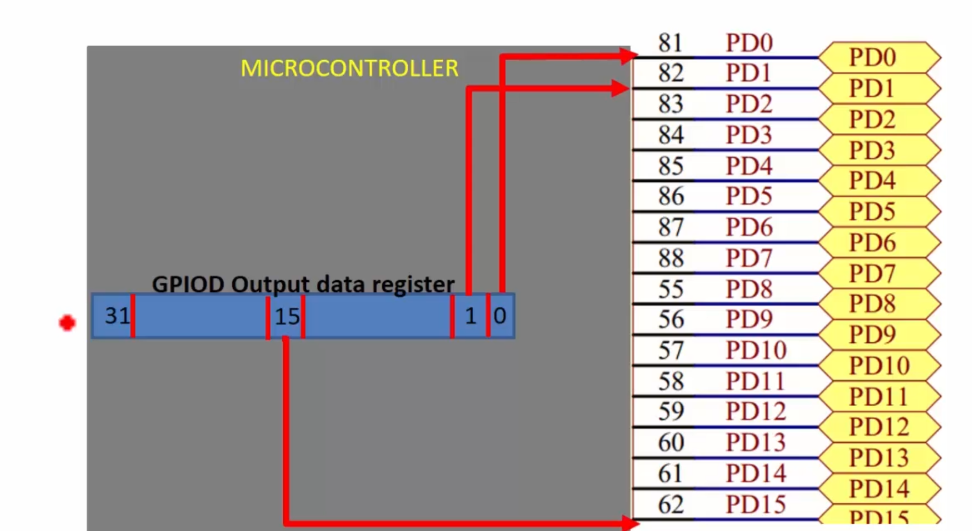
\includegraphics[scale=0.7]{Figures/Embedded_C/gpio_d_data_registers}
\caption{GPIOD Output Data Register}
\label{fig:Embedded_C:gpio_d_data_registers}
\end{figure}  

\end{itemize}

We will explore these registers later though coding and exercises.

\subsection{Procedure for turning a LED}

To turn a LED ON or OFF in a microcontroller, several thing need to be done and checked.

\begin{enumerate}
    \item Identify the GPIO port (peripheral) which LED is connected: port D
    
    \item In this port, which pin we will use  
    
    \item \tbi{Important: Enabling the pins}
    
    By default, in most microncontrollers, most pins are dead (in sleep mode). We must first activate the clock into them, otherwise no configuration or any operation can be performed.
    
    \begin{itemize}
        \item In some microcontrollers it can be otherwise, so we must check the data sheet before
        
        \item In stm microcontroller, all peripheral are in sleep mode and clock need to be configured
    \end{itemize}
    
    
\item Configure its mode (input pin or output pin)  

\item Write data to it
    
\end{enumerate}

It  is important to note that step 3 (enabling the clock) comes before step 4 (configuring the mode), otherwise we can't do anything. So in the next section we will learn how to configure the clock.

\newpage
\subsection{Configuring Clocks}

In stm32 microcontroller, most clock are configured through the \verb|RCC| register, which stands for reset and clock control. It can be found in chapter 6 in the reference manual.\\

Now the \verb|RCC| has many registers, and we are interested in configuring the clock relative to our peripheral, which is \verb|GPIO D|.\\

For \verb|GPIO D|, we need to use the \verb|RCC AHB1| bus register, because \verb|GPIO D| uses \verb|AHB1| bus to talk with the ARM microprocessor as shown in \autoref{fig:Embedded_C:gpio_d_ahb1_bus}.


\begin{figure}[h]
\centering
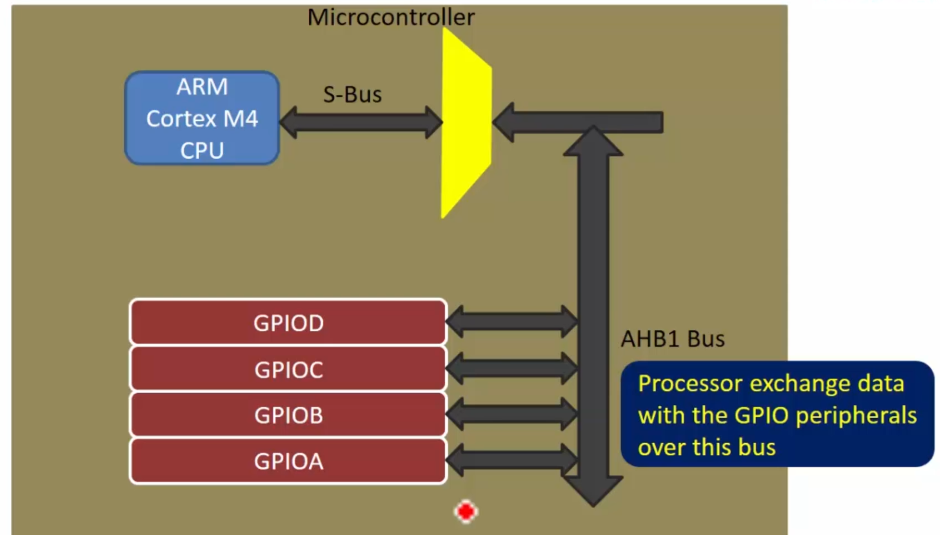
\includegraphics[scale=0.7]{Figures/Embedded_C/gpio_d_ahb1_bus}
\caption{GPIOD and AHB1 bus}
\label{fig:Embedded_C:gpio_d_ahb1_bus}
\end{figure}

This information we can know it from the \tbi{data sheet}, section 2.2 functional overview page 19. In \autoref{fig:Embedded_C:data_sheet_stm32407g_dis}, we have a screen shot of the diagram contained in the data sheet.

\begin{figure}[h]
\centering
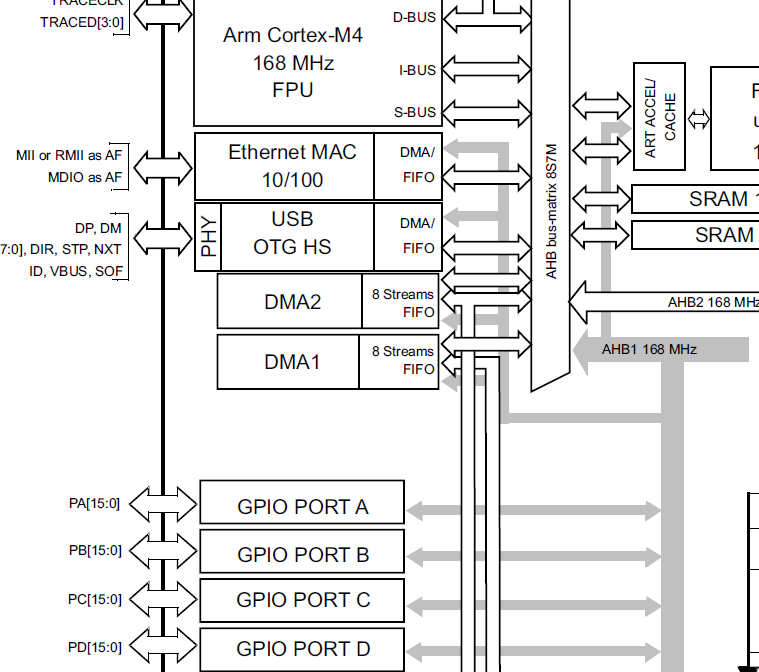
\includegraphics[scale=0.7]{Figures/Embedded_C/data_sheet_stm32407g_dis}
\caption{GPIOD and AHB1 bus}
\label{fig:Embedded_C:data_sheet_stm32407g_dis}
\end{figure}

As we can see, the \verb|GPIO D| uses \verb|AHB 1| bus to talk the ARM processor.\\

Now we understood which \verb|RCC| register is used for \verb|GPIO D|, we open the \textit{reference manual} to see how to set the \verb|RCC AHB1|. \verb|RCC AHB1| register is composed from several register (from section 6.3.5 $\rightarrow$ 6.3.10). Since we are interested in a clock configuration, we go to section 6.3.10, where we have clock options.

For \verb|GPIO D|, we need to set bit 3 (because it is written \verb|GPIO D EN|).

Address offset 0x30 means we need to add 30 to the base address of the \verb|RCC| to get to the \verb|RCC AHB1ENR| register.

The base address of the \verb|RCC| can be found the memory map section of the reference manual

\subsection{Configuring GPIO}

After setting the clock using the \verb|RCC| register, we need now to configure GPIO registers. For this application, we need to access 2 register:

\begin{enumerate}
    \item \verb|GPIOx MODER| (see section 8.4.1 in reference manual).
    
    \begin{itemize}
        \item Each 2 bits in this register is associated to 1 pin. This is because we have 4 state for each pin
        
        \item We are using LED on pin 12 of port D, so we need to assign 01 to bits 24 and 25 (responsible for pin 12).
        
        \item To do this, we can first clear bits using \verb|&| masking, then set the $24^\mathrm{th}$ bit to 1 using a bit wise OR mask
        
    \end{itemize}
    

\item After configuring pin type, we need to send output so the LED blink, and this is done using \verb|GPIOx ODR| rigister (see section 8.4.6)

\begin{itemize}
    \item Here we have 16 bits, which are enough to control the pins (either ON or OF, so 1 bit is enough to code these 2 states)
    
    \item We do it using a bit wise OR mask at bit 12
    
\end{itemize}
    
\end{enumerate}


\newpage
\subsection{Monitoring Registers in Real time}
\label{Sub:Registers_real_time_debug}

The smt32 cube IDE let us view real time application of the register.\\

To track the register in real time:

\begin{enumerate}
    \item We go in debug mode \verb|Debug As --> Stm32 C/C++ Application|
    
    Debugger mode will be on.
    
    \item From the tab menu, we go to \verb|Window --> Show View --> SFR|. A new window will appear at the right containing the registers as shown in \autoref{fig:Embedded_C:debug_registers_real_time}
    
    \begin{figure}[h]
\centering
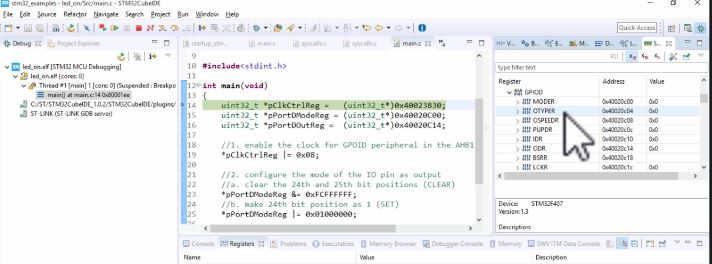
\includegraphics[scale=0.7]{Figures/Embedded_C/debug_registers_real_time}
\caption{Tracking registers in real time}
\label{fig:Embedded_C:debug_registers_real_time}
\end{figure}
    
    
\end{enumerate}





\newpage
\section{Bitwise Operation: shifting}

In \autoref{Sec:Led_practice}, we have done several register manipulation, that is set and clear bits in registers using port masking. This approach become very tedious, because each time \tbi{we need to  harcode the mask ourself}.

To avoid such a complication, we can use shifting operation.

\underline{Note:} \ref{sub:BitwiseLeft_app} contains the complete example wrap up.

\subsection{Bitwise Right}

Take the number a = $111_{10} = 6 F_{16} = 0110 1111$. Shifting by 4 bits is shown in \autoref{fig:Embedded_C:bitwise_shift_right_example}.

\begin{figure}[h]
\centering
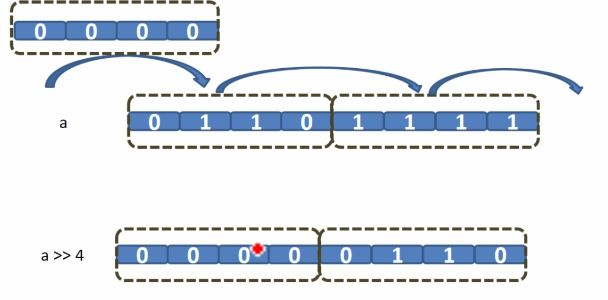
\includegraphics[scale=0.7]{Figures/Embedded_C/bitwise_shift_right_example}
\caption{Bitiwise shift: right direction by 4 bits}
\label{fig:Embedded_C:bitwise_shift_right_example}
\end{figure}

The result is $06_{16} = 6_{10}$.

\subsection{Bitwise Left}

We take same example in \autoref{fig:Embedded_C:bitwise_shift_right_example}, but with left direction this time. Example is shown in \autoref{fig:Embedded_C:bitwise_shift_left_example}.

\begin{figure}[h]
\centering
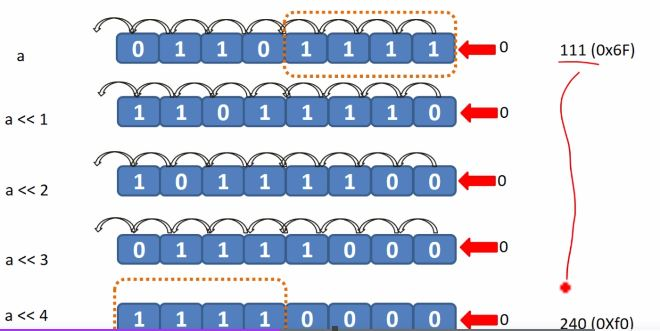
\includegraphics[scale=0.7]{Figures/Embedded_C/bitwise_shift_left_example}
\caption{Bitiwise shift: left direction by 4 bits}
\label{fig:Embedded_C:bitwise_shift_left_example}
\end{figure}

\newpage
\subsection{Some notes about bitwise shift}

In \autoref{fig:Embedded_C:bitwise_shift_note},we have a comparison table between bitwise shift left and right.

\begin{figure}[h]
\centering
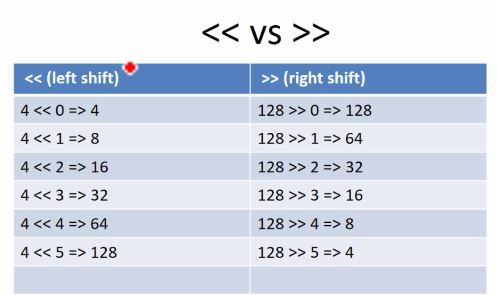
\includegraphics[scale=0.7]{Figures/Embedded_C/bitwise_shift_note}
\caption{Bitiwise shift: Left and Right Comparison}
\label{fig:Embedded_C:bitwise_shift_note}
\end{figure}

Shifting left increase the value, whereas shifting right decrease the  value by 2.

The reason behind this is the weight changing: when shifting to the left, the weights value increase, whereas in shifting to the right, the weight value of the number decrease.

\newpage
\subsection{Applicability of Bitwise in Embedded Programming}
\label{sub:BitwiseLeft_app}

Bitwise shift are very useful when clearing and setting bits in a given data register. We give 2 example for setting and clearing a bit.\\

\underline{Note:} 

\begin{itemize}

\item from now on, we use the new approach instead of the old one, that is figure out the value of the mask 

\item See code \verb|LED Bitshift| version to see the modification done.


\end{itemize}

Now we start the examples.

\begin{enumerate}
    \item \underline{Setting $4^\mathrm{th}$ bit}: In \autoref{fig:Embedded_C:bitwise_shift_set_bit}, we have the example using the old method and bitwise method
    

\begin{figure}[h]
\centering
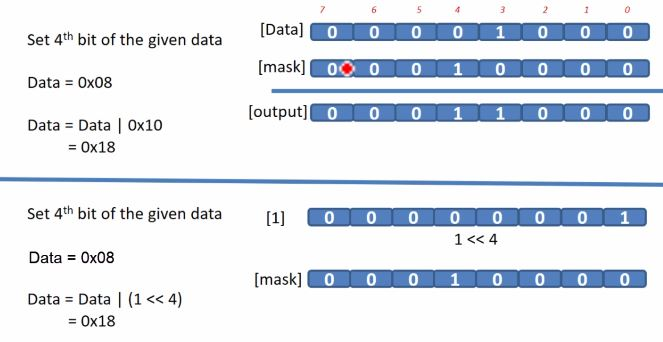
\includegraphics[scale=0.7]{Figures/Embedded_C/bitwise_shift_set_bit}
\caption{Bitiwise shift to set a bit}
\label{fig:Embedded_C:bitwise_shift_set_bit}
\end{figure}

	\begin{itemize}
	\item Note that using the \verb|1<<4| method, we don't need to figure out the value of the mask as in the old approach
	\end{itemize}
    
    
    
    \item \underline{Clearing a bit:}
    
    
    \begin{figure}[h]
\centering
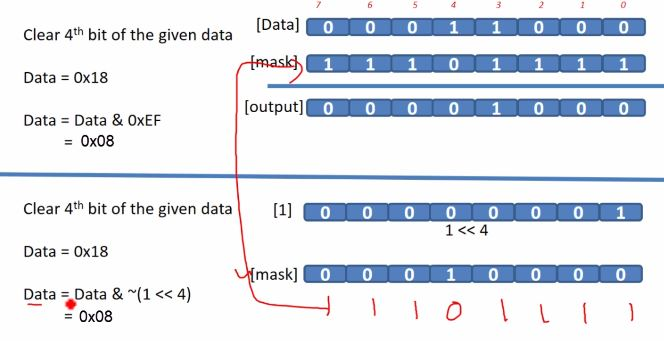
\includegraphics[scale=0.7]{Figures/Embedded_C/bitwise_shift_clear_bit}
\caption{Bitiwise shift to clear a bit}
\label{fig:Embedded_C:bitwise_shift_clear_bit}
\end{figure}
    
    
    Notice that after negating, the value will be the same as in the $\mathrm{1}^\mathrm{st}$ method
    
\end{enumerate}

 \underline{Note:} 

\newpage
\section{Bit Extraction}
\label{Sec:Bit_Extraction}

Now before we continue we present another task usually done in embedded programming called \textit{bit extraction}.\\


\underline{Problem Statement:} Extract bit position from $9^{\mathrm{th}} \rightarrow 14^{\mathrm{th}}$ bit position. The example is shown in \autoref{fig:Embedded_C:bit_extraction_problem}, along with the method used.

\begin{figure}[h]
\centering
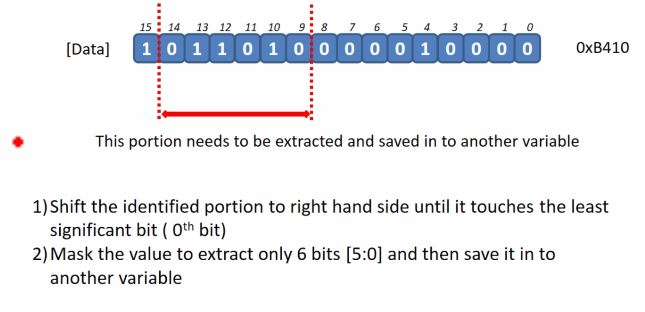
\includegraphics[scale=0.7]{Figures/Embedded_C/bit_extraction_problem}
\caption{Bit Extraction}
\label{fig:Embedded_C:bit_extraction_problem}
\end{figure}

The shifting step is shown in \autoref{fig:Embedded_C:bit_extraction_shifting}.

\begin{figure}[h]
\centering
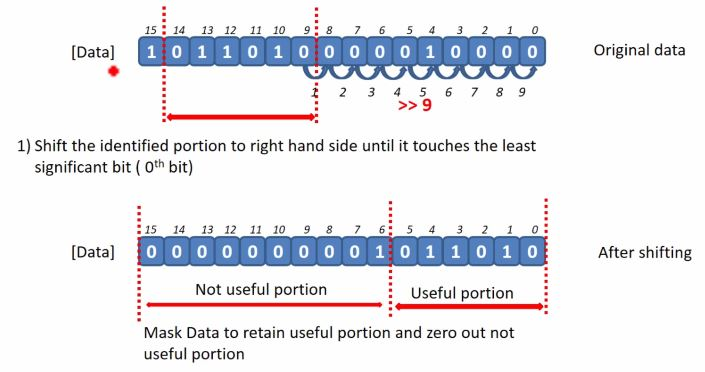
\includegraphics[scale=0.7]{Figures/Embedded_C/bit_extraction_shifting}
\caption{Bit Extraction: Shifting Step}
\label{fig:Embedded_C:bit_extraction_shifting}
\end{figure}


\newpage
Then after shifting we do masking to the shifted data as shown in \autoref{fig:Embedded_C:bit_extraction_masking}.

\begin{figure}[h]
\centering
\includegraphics[scale=0.7]{Figures/Embedded_C/bit_extraction_masking}
\caption{Bit Extraction: Masking the shifted data step}
\label{fig:Embedded_C:bit_extraction_masking}
\end{figure}


\underline{Code:}
\begin{itemize}
    \item \verb|uint16 t = 0xB410|
    
    \item  \verb|uint8 t output |
    
    \item \verb|output = (uint8 t)((Data >> 9)&0x003F)|
    
\end{itemize}


\newpage

\section{Loop in Embedded programming}

In this section, we explain some point and some pitfalls about loop in embedded programming.

\subsection{while loop}

\begin{enumerate}
    
    \item \verb|while| loop and the \verb|;|: We should pay attention in programming, when we put a \verb|;| after a \verb|while| loop.
    
    We have an example in \autoref{fig:Embedded_C:while_loop_note_1}.
    
    \begin{figure}[h]
\centering
\includegraphics[scale=0.7]{Figures/Embedded_C/while_loop_note_1}
\caption{while loop and semicolone}
\label{fig:Embedded_C:while_loop_note_1}
\end{figure}

It is clear that inserting a \verb|;| after the \verb|while| loop in this case will not make the counter to increment the variable \verb|i|.\\

 \item Super loop (forever loop): 
 
 In embedded programming unlike pc program, the program in the microcontroller need to run forever (or as long it is power up). In \autoref{fig:Embedded_C:while_loop_note_2}, we have an example of \verb|while| loop where the \verb|;| is inserted in the right place.
    
\begin{figure}[h]
\centering
\includegraphics[scale=0.7]{Figures/Embedded_C/while_loop_note_2}
\caption{while loop and semicolone}
\label{fig:Embedded_C:while_loop_note_2}
\end{figure}    
    
\newpage    
Another example is shown in \autoref{fig:Embedded_C:while_loop_note_3}   
   
\begin{figure}[h]
\centering
\includegraphics[scale=0.7]{Figures/Embedded_C/while_loop_note_3}
\caption{Super loop}
\label{fig:Embedded_C:while_loop_note_3}
\end{figure}     
    
\end{enumerate}

\subsection{do while}

Unlike the \verb|while| which can or can't have a \verb|;|, a \verb|do while| \tbi{must have a } \verb|;| after it, otherwise it will be a compilation error.

In embedded programming, we use \verb|do while| loop when writing \textit{multiline C macros in a header file}. This part will be explored later when we talk about macros and header file in later sections.

\newpage
\section{LED Toggling}
\label{Sec:LED_Toggling}

In this section, we will modify the LED ON program to produce a toggling LED. The purpose is to use start using loops in a embedded programming.\\

\underline{Problem Statement:} write a program to make the LED toggle between ON and OFF state, where a certain \textit{delay} is injected between these 2 states.\\

\underline{Delay types:} to produce a certain delay, we have 2 methods:

\begin{enumerate}
    
    \item software method: this done using \verb|for| loop for example. However, this method is inaccruate and waist allot of cycles.
    
    \item Hardware method: this is done using peripheral such as timers. This method is more accurate.

\end{enumerate}

For the LED toggling application, we will use software method since accuracy is not important in this application. We are only interested to produce a human observable delay to see the toggling.\\

See project \verb|LED Toggling|.

\newpage
\section{Type Qualifier: const}
\label{Sub:const_type_qualifier}

The first qualifier we encounter is \verb|const|. When used in front of variable, this means we can real only but not modified. Nevertheless, we can still modify the value by accessing the address via pointer as shown in \autoref{fig:Embedded_C:const_and_pointer}.

\begin{figure}[h]
\centering
\includegraphics[scale=0.9]{Figures/Embedded_C/const_and_pointer}
\caption{Changing a const variable via pointer}
\label{fig:Embedded_C:const_and_pointer}
\end{figure}   

Also, there exist several cases, which are illustrated in \autoref{fig:Embedded_C:const_usage_case}.

\begin{figure}[h]
\centering
\includegraphics[scale=0.5]{Figures/Embedded_C/const_usage_case}
\caption{const usage case}
\label{fig:Embedded_C:const_usage_case}
\end{figure} 

\newpage
For the $1^{\mathrm{st}}$ case, an example is shown \autoref{fig:Embedded_C:const_fixed_data_change_ptr}.

\begin{figure}[h]
\centering
\includegraphics[scale=0.7]{Figures/Embedded_C/const_fixed_data_change_ptr}
\caption{const case: modifiable pointer and constant data }
\label{fig:Embedded_C:const_fixed_data_change_ptr}
\end{figure} 

The goal is to protect the data contained in the source from being modified accidentally.\\

As for the $2^{\mathrm{nd}}$ case, example shown in \autoref{fig:Embedded_C:const_fixed_ptr_change_data}.

\begin{figure}[h]
\centering
\includegraphics[scale=0.7]{Figures/Embedded_C/const_fixed_ptr_change_data}
\caption{const case: modifiable data and constant pointer }
\label{fig:Embedded_C:const_fixed_ptr_change_data}
\end{figure} 

\newpage
Last case is shown in \autoref{fig:Embedded_C:const_all_fixed}

\begin{figure}[h]
\centering
\includegraphics[scale=0.7]{Figures/Embedded_C/const_all_fixed}
\caption{const case: all is fixed}
\label{fig:Embedded_C:const_all_fixed}
\end{figure} 



\begin{itemize}
    \item \verb|const* src|: the programmer know that the content pointed by \verb|src| should not be modified
    
    \item Several cases for the usage of \verb|const| qualifier
    
    
\end{itemize}


\newpage    
\section{Pin read}
\label{Sec:Pin_read}

Now we will do another exercise to practice more.

\subsection{Problem Statement}

Write a program which read the status of pin \verb|PA0|. If \verb|PA0| is high, then the LED pin \verb|PD12| (used in exercises before) is ON, and if \verb|PA0| is low, then \verb|PD12| is OFF.\\

Change the status of \verb|PA0| manually by connecting between \verb|GND| and \verb|VDD| points of the board.

\subsection{Hints and Checking}

When dealing with such program, the $1^\mathrm{st}$ thing we need to do is to check whether \verb|PA0| if a free IO pin or not. In smt32407g discovery board, usually it is. \\

To know that, we open the \textit{user manual} at table 7 in chapter 6. We see at the row containing \verb|PA0|, the column named free IO pin contain \verb|PA0|, so we can use \verb|PA0| as free IO pin.

For other pins at port A, it is not necessary the case. For example, the \verb|PA4| row, the free IO column is empty, sow can't use \verb|PA4| as free IO pin.

\subsection{Programming}

Now in this exercise, we have 2 ports: A and D. 

For port A, we should read from it so it is considered as input.\\

Also, we need to enable the clock for port A the same way we did for port D in the LED exercise. We use also the same register (\verb|RCC AHB1ENR|) because all \verb|GPIO| peripheral use \verb|AHB1| bus. For \verb| GPIO D|, the pin we set was pin 3, and for \verb|GPIO A| it could be a different pin, so we need to check the \textit{reference manual} (section 6.3.10, it will be pin 0 for GPIO A).\\

To configure \verb|PA0| as input, we need to access $\mathrm{1}^\mathrm{st}$ the \verb|GPIO-A| base address (see section 2.3 memory map in the reference manual) the same way we did for \verb|GPIO-D|, then setting the input mode via \verb|GPIO MODE| register.

Once we configured \verb|PA0| as input, we need to read from it voltage values (\verb|GND| or \verb|VDD|). In the LED exercise, we used the \verb|GPIO ODR| to write values to the LED, and here we will use \verb|GPIO IDR| (input data register, see section 8.4.5 in the reference manual).


\newpage
\section{Compiler Optimization}

Before continuing in the next features of embedded C, the \verb|volatile| concept, we need $\mathrm{1}^\mathrm{st}$ to understand optimization concepts done by the compiler.\\

Optimization is a series of actions taken by the compiler on our written embedded code to:

\begin{itemize}
    \item number of instruction (code space optimization)
    
    \item Memory access time (time space optimization)
    
    \item Power consumption
    
\end{itemize}

By default, compiler doesn't do any optimizaiton, but we can enable optimization using \textit{flags}. Different flags exist: \verb|-O0|, \verb|-O1 --> -O3|.\\

The \verb|-O0| is the phase were no optimization is done. The benefits of it:

\begin{itemize}
    \item debugging friendly (for each code, 1 assembly instruction is generated)
    
    \item fast at compilation time.
\end{itemize}

However, it is not recommended for application constrained by their space or RAM. \\

The other flags are quite the opposite: more efficient but less friendly debugging, and take longer time to compile. Each level has its own sophistication and features, and we need to use them depending on our application and needs (no specific guideline about them).

\newpage
\subsection{Pin Read Optimization}
\label{Sub:Pin_Read_Optimization}

As a concrete example how compiler optimization can effect our code, we will retake the \verb|Pin read| exercise, and set the IDE to 2 different compilation mode flag: \verb|-O0| and \verb|-O2|.\\

\underline{\texttt{-O2} Level:}

In \autoref{fig:Embedded_C:pin_read_O0_flag}, we have the disassembly equivalent code of line 37

\begin{figure}[h]
\centering
\includegraphics[scale=0.7]{Figures/Embedded_C/pin_read_O0_flag}
\caption{Pin read demo: -O0 optimization}
\label{fig:Embedded_C:pin_read_O0_flag}
\end{figure} 

The \verb|pinStatus| variable value is loaded successfully at each seconds during the \verb|while| loop. This essential to our pin reading application because we need to be able to check at every time moment the status of the pin, so we can turn ON or OFF the led \verb|PD12|.\\

\underline{\texttt{-O2} Level:}\\

Now when switching compilation mode to \verb|-O2|, line 17 will not be break down in a 1-to-1 disassembly code as in \autoref{fig:Embedded_C:pin_read_O0_flag}. That is because the compiler will add some optimization algorithm to reduce either time space or code space. The correspondent disassembly program to \verb|-O2| is shown in \autoref{fig:Embedded_C:pin_read_O2_flag}.

\newpage
\begin{figure}[h]
\centering
\includegraphics[scale=0.7]{Figures/Embedded_C/pin_read_O2_flag}
\caption{Pin read demo: -O2 optimization}
\label{fig:Embedded_C:pin_read_O2_flag}
\end{figure} 

\begin{itemize}
    \item In debug mode, the execution of the code is random and not line by line as in \verb|-O0|. 
    
    This is because the compiler is generating some instruction to do optimization
    
    \item When reaching the \verb|while| loop, the compiler will not execute line 17 anymore.
    
    The reason is so he can optimize time, by reducing memory hit and not reading the \verb|pinStatus| value in the memory.

\end{itemize}

It is true it is maybe an optimization in time, but now the application is not working.\\

So the question to arise: how we can prevent compiler from doing unwanted optimization to our code? here it comes the role \verb|volatile|.

\newpage
\section{Volatile Type Qualifier}

\verb|volatile| is type qualifier which tells the compiler to not do any optimization on the variable operation (read and write).

It also tells the compiler that the value of the variable may change at any time with or without programmer consent. So it turns off optimization on variable operation (read and write).\\

Let's take another example to see compiler optimization. In , we have some code along with the assembly code, at \verb|-O0| optimization level.

\begin{figure}[h]
\centering
\includegraphics[scale=0.7]{Figures/Embedded_C/demo_O0_flag}
\caption{Demo -O0 optimization}
\label{fig:Embedded_C:demo_O0_flag}
\end{figure} 

Notice that although we have redundant instruction (so instruction optimization can be performed), compiler generate all the assembly code, even for the redundant instruction, that's because we are in \verb|-O0| level.\\


\newpage
Now suppose we use \verb|-O1| level (shown in \autoref{fig:Embedded_C:demo_O1_flag}), compiler won't generate anything except for the \verb|for(;;)| statement 

\begin{figure}[h]
\centering
\includegraphics[scale=0.7]{Figures/Embedded_C/demo_O1_flag}
\caption{Demo -O1 optimization}
\label{fig:Embedded_C:demo_O1_flag}
\end{figure} 

The compiler did this because it is true we declare and initialize the variables, but we didn't use them at all (we didn't do any operation, pass them to some function,$\cdots$).\\


If we don't want any optimization, we use the \verb|volatile| type qualifier as shown in \autoref{fig:Embedded_C:demo_O1_volatile}

\begin{figure}[h]
\centering
\includegraphics[scale=0.7]{Figures/Embedded_C/demo_O1_volatile}
\caption{Demo -O1 optimization with volatile}
\label{fig:Embedded_C:demo_O1_volatile}
\end{figure} 

Notice that now even if we are in \verb|-O1| (or higher) levels, the compiler generate all assembly instructions.\\

\underline{Note:} Type qualifier (such as \verb|const| and \verb|volatile|) comes always after type specifier (\verb|uint8 t|).


\subsection{Use case of volatile}

The \verb|volatile| is used whenever there is a possibility to a variable to be changed (change can be coming from software or Hardware).\\

In embedded system context, here the 3 cases where \verb|volatile| should be used:

\begin{enumerate}
    \item Memory mapped peripheral registers of the micrcocontroller (as in the pin read exercise in \ref{Sub:Pin_Read_Optimization})
    
    \item Multiple tasks accessing global variables (read/write) in an RTOS multithreaded application
    
    \item When a global variable is used to share data between the main and an ISR code
    
\end{enumerate}

\subsection{volatile different syntax}

As in the case \verb|const| different syntax meaning (\autoref{Sub:const_type_qualifier}), same thing exist for \verb|volatile| type qualifier. \autoref{fig:Embedded_C:volatile_syntax} shows the different use case for \verb|volatile|

\begin{figure}[h]
\centering
\includegraphics[scale=0.55]{Figures/Embedded_C/volatile_syntax}
\caption{volatile syntax use cases}
\label{fig:Embedded_C:volatile_syntax}
\end{figure} 

\begin{itemize}
    
    \item Case 2 is the most used case in embedded programming: we use it whenever we access memory mapped register
    
    \item Case 3 and 4 are rarely used

\end{itemize}

\subsection{volatile and ISR}

In this section, we explore the usage of \verb|volatile| with ISR (interrupt service routine).\\

\underline{Note: IDE usage:} To see how the counter is increased every time we press the button, we go to debug mode, and then run the code using the green arrow, and set the console at \verb|SWV ITM Data Console| as shown in \autoref{fig:Embedded_C:IDE_swv_push_button}.


\begin{figure}[h]
\centering
\includegraphics[scale=0.55]{Figures/Embedded_C/IDE_swv_push_button}
\caption{IDE usage: SWV console for counter using push button}
\label{fig:Embedded_C:IDE_swv_push_button}
\end{figure}

Make sure that port0 is checked (as shown in \autoref{fig:Embedded_C:IDE_swv_push_button_port_0}).

\begin{figure}[h]
\centering
\includegraphics[scale=0.55]{Figures/Embedded_C/IDE_swv_push_button_port_0}
\caption{IDE usage: SWV console for counter using push button}
\label{fig:Embedded_C:IDE_swv_push_button_port_0}
\end{figure}



\todo{IDE:} 

\begin{itemize}
    
    \item \textit{To explore later why we need to check port0 is checked}
    
    \item \textit{This technique can be used in debugging our application}
    
\end{itemize}


\newpage
\section{Structure and Bit Field}
\label{Sec:Structure_bit_field}

\subsection{Some Key Concepts}

\begin{itemize}
    \item structures are usually defined in header file or outside the \verb|main| function
    
    Review from C book how to create (declare) initialize and access structures.
    
    \todo{C book Reference:} \underline{\textit{C book Reference}:} \textit{To include C book reference} 
    
    
    \item Padding concept in structure:
    
    \begin{itemize}
        \item compiler doesn't store variable values at arbitrary addresses, rather it stores them in a way such that the end of each variable address correspond to natural boundary of the variable data type.
        
        
        \item As example, consider \autoref{fig:Embedded_C:struture_padding_example_1} where we have 3 data types: \verb|char| (consume 1 byte), \verb|int| (consume 4 byte) and \verb|short|(consume 2 byte).
        
        \begin{figure}[h]
\centering
\includegraphics[scale=0.55]{Figures/Embedded_C/struture_padding_example_1}
\caption{Structure padding example}
\label{fig:Embedded_C:struture_padding_example_1}
\end{figure}

Notice the end of each address. For \verb|char|, the end of address can be 0,1,2,$\cdots$ because \verb|char| consume 1 byte.

For \verb|short|, it can be 0, then 2 (and not 1), then 4,$\cdots$, because \verb|short|consume 2 byte.

    \end{itemize}
    

\item Packed Structure allow more efficient communication between the microcontroller and the memory (Use less assembly code for each member initialization of a structure member. Less assembly means less clock cycles)

\todo{Packed code demo} \underline{ \textit{Packed code demo}:} 

\begin{itemize}
    \item \textit{See demo} \verb|packed vs Unpacked| \textit{and compare the assembly code}.

    \item \textit{to run the code and document it, along with structure demo}.
    
\end{itemize}

\item When using a \textit{pointer of type structure}, such as \verb|struct Dataset *pdata| (where the initial structure is \verb|struct Dataset data|, and \verb|data| is an instance), we use the arrow operator \verb|->| to access/set members (\verb|pdata-> date = 12|).

If we deal with normal structure variable, we use \verb|.| operator (\verb|data.date = 12|)

\end{itemize}

\newpage
\subsection{Packet Exercise}
\label{Sub:Packet_Exercise}

\underline{Concepts used:}

\begin{itemize}
    \item Bit extraction, mask and bit shift operation (Review \autoref{Sec:Bit_Extraction})
\end{itemize}

\underline{Problem Statement:} Enter some 32 bit packet value in Hexadecimal. The composition of the packet is shown in \autoref{fig:Embedded_C:packet_exercise}. Print the value of each section in this packet.


\begin{figure}[h]
\centering
\includegraphics[scale=0.7]{Figures/Embedded_C/packet_exercise}
\caption{packet exercise: problem statement}
\label{fig:Embedded_C:packet_exercise}
\end{figure}


\underline{Note:} For hexadecimal with \verb|scanf|, we use \verb|%X|.

\todo{Bit,byte,...} \textit{Insert a table of definition bit,byte, hexa and different base number format (from digital design course)}\\

\underline{Project:} See \verb|Packets| and \verb|Packets bit fields|.



\newpage
\section{Union}
\label{Sec:union}

Unions are variables which share the same memory location. An example is shown in \autoref{fig:Embedded_C:union_example}.


\begin{figure}[h]
\centering
\includegraphics[scale=0.7]{Figures/Embedded_C/union_example}
\caption{Union Example}
\label{fig:Embedded_C:union_example}
\end{figure}

\begin{itemize}
    \item We define the union the same way we define a structure: we just replace the keyword \verb|struct| by \verb|union|
    
    \item The size of a union is equal to the size of its largest members
    
    \begin{itemize}
        \item In the example of \autoref{fig:Embedded_C:union_example}, the size will be 4 byte
    \end{itemize}

\end{itemize}

We usually use the union whenever the member usage is \tbi{mutually exclusive}, that is we only use 1 of them at a time.\\

\todo{Union Demo} \underline{\textit{Union Demo}:} 

\begin{figure}[h]
\centering
\includegraphics[scale=0.7]{Figures/Embedded_C/union_demo_overwritten}
\caption{Union demo: overwritten values}
\label{fig:Embedded_C:union_demo_overwritten}
\end{figure}

\begin{itemize}
    \item \textit{Write the code of union demo} 
    
    \item \textit{In union, we will see that we have variable overwritten}
    
    \item \textit{since both members share the same memory location, the longaddr will overwrite the short addr, that's why we don't see 0xABDC}
\end{itemize}


\subsection{Applicability of Union in embedded programming}

Now we will do the packet exercise (see \ref{Sub:Packet_Exercise}) using a combination of \verb|union| and \verb|struct| implementation.\\

\todo{Union Packet Exercise} \underline{\textit{Union Packet Exercise}:}

\begin{itemize}
    \item \textit{Create a project, and repeat the packet exercise} 
    
    \item \textit{Compare the output and write note and explanation} 
\end{itemize}


\begin{figure}[h]
\centering
\includegraphics[scale=0.55]{Figures/Embedded_C/union_packet_exercise}
\caption{Union Packet Exercise}
\label{fig:Embedded_C:union_packet_exercise}
\end{figure}

\underline{Project:} See \verb|Packets Union struct version| in \verb|Host|

\newpage
\section{Bit fields in Embedded Code}

Bit fields and structure are heavily used in embedded programming to present abstraction when dealing with code. We will use these concepts by refactoring the LED toggling exercise (see \autoref{Sec:LED_Toggling}).\\

For example, in the \verb|LED Toggle| project, we use the \verb|RCC-AHB1ENR| (shown in \autoref{fig:Embedded_C:RCC_peripheral_AHB1_Reg}) to enable the clock for the \verb|GPIO-D| (since we are using LED on \verb|port D|). This is implement it via the following \verb|C| command: *clck-register|=  1<<3. The only way we can know that we need shift left via position 3 is if we have a reference manual at our side.


\begin{figure}[h]
\centering
\includegraphics[scale=0.55]{Figures/Embedded_C/RCC_peripheral_AHB1_Reg}
\caption{RCC Peripheral with its corresponding AHB1 register}
\label{fig:Embedded_C:RCC_peripheral_AHB1_Reg}
\end{figure}

In setting this register, we used bit shift and masking operation. Now we will use bit fields and structure to abstract these low level operation, and make our code more usable by other users.\\

\underline{Prerequisite:}

\begin{itemize}
    \item \autoref{Sec:LED_Toggling}
    
    \begin{itemize}
        \item Review the concept of bit shift, accessing register concept, because we will do abstraction implementation and eliminate all the details, and then \textit{compare both implementation}
    \end{itemize}
    
    \item Structures \autoref{Sec:Structure_bit_field} and Unions \autoref{Sec:union}
    
\end{itemize}


\underline{Project Demo:} See \verb|Led Toggles Bit Fields|.\\

\newpage
\underline{Some Notes:}

\begin{itemize}
    \item In the \verb|.h| file: don't forget to include \verb|stdint.h|
    
    \item Compile the header file which contains all the defined structure (by doing right click on \verb|.h| file then \verb|Build project|) directly to see if there is an error in the \verb|.h| file.
    
    
    \item Once we create the \verb|typedef struct| which encode different register, \autoref{fig:Embedded_C:led_toggl_bit_fields_encode_register} shows the implementation and what happen inside the compiler
    
    \begin{figure}[h]
\centering
\includegraphics[scale=0.55]{Figures/Embedded_C/led_toggl_bit_fields_encode_register}
\caption{Structure implementation and encoding for register}
\label{fig:Embedded_C:led_toggl_bit_fields_encode_register}
\end{figure}
    
    
\end{itemize}

\newpage

\section{Keypad Interfacing}

In this section we will implement another project for practice: matrix keypad and interface it with the stm microcontroller.\\

In \autoref{fig:Embedded_C:keypad_matrix}, we have the keypad along with its connection.

\begin{figure}[h]
\centering
\includegraphics[scale=0.55]{Figures/Embedded_C/keypad_matrix}
\caption{Keypad}
\label{fig:Embedded_C:keypad_matrix}
\end{figure}


\begin{itemize}
    \item The R1 $\rightarrow$ R4 are called row lines, and C1 $\rightarrow$ C4 are column lines

    \item Inside the keypad, we have different keys which connect R and C.

    \item When the key is not pressed, there is no connection between R and C lines, and otherwise (key is pressed) there will be a contact between a row and a column

    \item : C are input to the microcontroller, and R are output from microcontroller

\end{itemize}

A more detailed schematic of the keypad with each keys is shown in \autoref{fig:Embedded_C:keypad_matrix_each_key}.

\begin{figure}[h]
\centering
\includegraphics[scale=0.55]{Figures/Embedded_C/keypad_matrix_each_key}
\caption{Keypad with each different key}
\label{fig:Embedded_C:keypad_matrix_each_key}
\end{figure}


\newpage
In \autoref{fig:Embedded_C:keypad_connection_to_micro}, we have the connection of the keypad to the microcontroller.

\begin{figure}[h]
\centering
\includegraphics[scale=0.55]{Figures/Embedded_C/keypad_connection_to_micro}
\caption{Keypad connection with the microcontroller}
\label{fig:Embedded_C:keypad_connection_to_micro}
\end{figure}


\begin{itemize}
    \item We need 8 \tbi{free IO pins} from the microcontroller

    \begin{itemize}
        \item We need to go to the reference manual to check whether the pin are free or not (same as we did in \autoref{Sec:Pin_read} with the pin read exercise)
    \end{itemize}

    \item Also we usually need some pull up resistors concerning the column part

    \begin{itemize}
        \item We can use the internal pull up resistors that come with the microcontroller. No need for extra resistors
    \end{itemize}

    
\end{itemize}

\subsection{Why Pull up resistors}

In \autoref{fig:Embedded_C:hand_sketch_key_MCU} we have a hand sketch of a key, connected to a MCU.\\

\begin{figure}[h]
\centering
\includegraphics[scale=0.55]{Figures/Embedded_C/hand_sketch_key_MCU}
\caption{Hand sketch of MCU and a Key}
\label{fig:Embedded_C:hand_sketch_key_MCU}
\end{figure}


When the key is not pressed, the circuit is in open state (open circuit), and hence the key (the pin at C1) can take several voltage values due to random noise coming from circuitry in the open state. This is called \textit{floating state}.\\

\todo{Open circuit:} \underline{\textit{Open circuit:}} \textit{To review later the concept of open circuit, and its relation to noise,$\cdots$}.\\

To avoid such floating state, we connect pull up resistor (it should be of high value) between the pin C and the Vcc as shown in \autoref{fig:Embedded_C:hand_sketch_key_MCU_pull_up}. We can also use pull down resistor between the pin and ground. 

After connecting the pull up resistor, the voltage at pin C is Vcc.\\

\begin{figure}[h]
\centering
\includegraphics[scale=0.55]{Figures/Embedded_C/hand_sketch_key_MCU_pull_up}
\caption{Hand sketch of MCU and a Key plus a pull up resistor}
\label{fig:Embedded_C:hand_sketch_key_MCU_pull_up}
\end{figure}

\todo{Voltage at pin C} \textit{Voltage at pin C}: \textit{To review later why this is the value. Need to review circuit analysis concepts.}\\

So now, whenever we read pin \verb|PD8| from the MCU, if the key is not pressed, the value will be high equal to Vcc.\\

\underline{So first rule:} when the key is not pressed (and off course there is pull up resistors), C is high, and the input status of MCU is high.\\

Now the next logical state is when the key is pressed, the C should be low. So here we use the output of MCU (because we can control it) and connect it to ground as shown in \autoref{fig:Embedded_C:hand_sketch_key_MCU_ground}. By this way, when key is pressed, C is connected to ground and the input MCU is low.\\

\begin{figure}[h]
\centering
\includegraphics[scale=0.55]{Figures/Embedded_C/hand_sketch_key_MCU_ground}
\caption{Hand sketch of MCU and a Key: output pin connected to ground}
\label{fig:Embedded_C:hand_sketch_key_MCU_ground}
\end{figure}


\underline{$\mathrm{2}^\mathrm{nd}$ Rule:} when the key is pressed, the value is low.



\newpage

\section{Preprocessor Directive}
\label{Sec:Preprocessor_Directive}

Preprocessor are the \verb|C| statements which begin with \verb|#| (such as \verb|#include|). They are used as textual replacement for numbers, and other things.

The important thing also is that these statements are taken care during the preprocessing stage of the compilation time, and instruct the compiler to do number of things.\\

In \autoref{fig:Embedded_C:preprocessing_directive_types}, we have different type of preprocessing directive

\begin{figure}[h]
\centering
\includegraphics[scale=0.55]{Figures/Embedded_C/preprocessing_directive_types}
\caption{Different type of preprocessing directives}
\label{fig:Embedded_C:preprocessing_directive_types}
\end{figure}

Now we start with each type of operation in the following subsections.

\subsection{Macros Preprocessor}

In \autoref{fig:Embedded_C:macros_syntax_example}, we have the syntax of a macros.

\begin{figure}[h]
\centering
\includegraphics[scale=0.55]{Figures/Embedded_C/macros_syntax_example}
\caption{Macros Syntax Example: Replace some constant}
\label{fig:Embedded_C:macros_syntax_example}
\end{figure}

Some important notes about macros:

\begin{itemize}
        \item There is a space between each word

        \item No \verb|;| is required to terminate the statement

        \item The macros are not variables: they are just textual replacement where this replacement takes place during compilation time 

        \item Use case in embedded programming: define pin number,pin values,crystal speed,peripheral register addresses,memory addresses,$\cdots$.\\

        \underline{Examples:} \verb|#define PIN-8 8|

        \verb|#define LED-STATE-ON 1|

        We use capital case to distinguish between variables and macros text.

        
    \end{itemize}


Another type of macro is the \tbi{function like macros}, where an example is shown in \autoref{fig:Embedded_C:macros_function}.

\begin{figure}[h]
\centering
\includegraphics[scale=0.55]{Figures/Embedded_C/macros_function}
\caption{Macros function}
\label{fig:Embedded_C:macros_function}
\end{figure}

However, it should be noted that the macros function shown in \autoref{fig:Embedded_C:macros_function}  is poorly written, because a user can use the macros as this for example:\verb|AREA-OF-CIRCLE(1+1)|.  Because now \verb|r = 1+1| and due arithmetic precedence, we will obtain a different area value then \verb|AREA-OF-CIRCLE(2)|.\\

To prevent this, we always use \verb|()| when we have function like macros with multiple operands and operations, as shown in \autoref{fig:Embedded_C:macros_function_2}.

\begin{figure}[h]
\centering
\includegraphics[scale=0.55]{Figures/Embedded_C/macros_function_2}
\caption{Macros function with ()}
\label{fig:Embedded_C:macros_function_2}
\end{figure}

\newpage
\subsection{Conditional Directive}

There exist several conditional directive. These are the follows:

\begin{itemize}
    \item \verb|#if|
    
    \item \verb|#ifdef|

    \item \verb|#endif| 

    \item \verb|#else|

    \item \verb|#undef|

    \item \verb|#ifndef|

\end{itemize}

The goal of these directive is to \tbi{include or exclude block of codes}. Let's start now with each directive.\\

\underline{ \#if and \#endif:}

Explanation is shown in \autoref{fig:Embedded_C:if_directive}

\begin{figure}[h]
\centering
\includegraphics[scale=0.55]{Figures/Embedded_C/if_directive}
\caption{\#if and \#endif}
\label{fig:Embedded_C:if_directive}
\end{figure}

\begin{itemize}
    \item We have to use constant

    \item When constant = 0 $\rightarrow$ code will not be included during build time
\end{itemize}


\newpage
Also, we can use \verb|#else| inside the \verb|#if|, as shown in \autoref{fig:Embedded_C:if_else_directive}.


\begin{figure}[h]
\centering
\includegraphics[scale=0.55]{Figures/Embedded_C/if_else_directive}
\caption{\#if and \#endif with \#else}
\label{fig:Embedded_C:if_else_directive}
\end{figure}

\begin{itemize}
    \item When constant = 1 $\rightarrow$ code block 1 will be build, and code block 2 will be excluded

    \item When constant = 0 $\rightarrow$ code block 2 will be build (inside the \verb|#else| block will be built), and code block 1 will be excluded

    
\end{itemize}

\underline{\#ifdef:}

The \verb|#ifdef| is different from \verb|#if| because we need to use a macros before the \verb|main| function, using the \verb|#define| operator. An example is shown in \autoref{fig:Embedded_C:ifdef_directive_example}.


\begin{figure}[h]
\centering
\includegraphics[scale=0.55]{Figures/Embedded_C/ifdef_directive_example}
\caption{\#ifdef preprocessor and \#define macros}
\label{fig:Embedded_C:ifdef_directive_example}
\end{figure}

\begin{itemize}
    \item There is a \verb|#end| at the last to terminate the block (not shown in \autoref{fig:Embedded_C:ifdef_directive_example})
\end{itemize}

So in other words, what \verb|#ifdef| is doing is if a certain feature (defined by a macros) is defined, then the block code will be executed.


\newpage
\section{Summary: Introduction and Embedded C}

\begin{enumerate}
    \item Each microcontroller contains several peripherals
    
    \begin{itemize}
        \item Each peripheral have different registers
        
        \item Each register has its own start and end address
        
        \item Addresses can be found in reference manual, section memory map
    \end{itemize}
    
\item Ports in stm32 usually have 16 pins

\begin{itemize}
    \item Used in connecting external hardware (display,button,Bluetooth transceiver,$\cdots$)
\end{itemize}

\item  Creating project: see \autoref{Sec:creating_project}.

\underline{Rules to remember regarding stm cube IDE:} 

\begin{itemize}

    \item  2 types of project we can create: 1 for host (\ref{sub:creating_project_for_host}) and 1 for target (\ref{Sub:Project on Board})

    \item Before creating a project, we need to create a workspace (see \ref{Sub:creating_workspace})
    
    \item Note that when finishing creating a workspace for some directory, we will a \verb|.metadata| folder associated with this workspace.


\end{itemize}

\item \ref{Sub:Registers_real_time_debug}: nice for debugging and monitoring registers in real time  

\item Structures (\autoref{Sec:Structure_bit_field}):

\begin{itemize}
    \item When to use \verb|->| and when to use \verb|.| operator (1 with pointer of type structure and the other normal structure instance)
\end{itemize}
    
\item Unions and structure: From the packet exercise (see \autoref{Sub:Packet_Exercise})

\begin{itemize}
    \item In \verb|Packet| project: learn how to compute mask value, and compute bit shift values. But this implementation consume more memory (Instead of 4 byte, it consumes 10 bytes due to structure padding)
    
    \item In \verb|Packet bit fields|: we use bit fields to do proper allocation (\textit{consume less memory})
    
    \item In \verb|Packets union struct version|: The we use union and struct implementation combined (nested implementation) to avoid bit shift operations and do direct assignment
    
 
\end{itemize}

\item Preprocessor Directives: \verb|C| statements which begin with \verb|#|, instruct the compiler to do certain things during the preprocessing stage in compilation time.\\

\underline{Rule to remember:} with function like macros: we always use \verb|()| when we have function like macros with multiple operands and operations.

To see more details review \autoref{Sec:Preprocessor_Directive}.
   
\end{enumerate}

\newpage
\subsection{Code Order}

Describing order of projects in \verb|stm32f4G-Discovery_Essentials| directory

\begin{enumerate}    
    
    \item \verb|LED|: turning ON LED

    \begin{itemize}
        \item Use mask computation in traditional way

    \end{itemize}

    \item \verb|LED-bitshift|: turning ON LED but \tbi{using bit shifting concepts}

    \begin{itemize}
        \item No mask computation
        
		\item  See \ref{sub:BitwiseLeft_app} for complete example.       
        
    \end{itemize}

\item \verb|LED Toggling|: Illustrate loop and delay concepts via software

    \begin{itemize}
        \item Not very important for now
    \end{itemize}


\item \verb|Packets|, \verb|Packets bit fields| and \verb|Packets union struct version|, in \verb|Host| workspace. 

Exercise given in \ref{Sub:Packet_Exercise}

\begin{itemize}
    \item \verb|Packets| demo: use normal structure definition (no allocation of bit fields)

    \begin{itemize}
        \item This cause in structure definition to allocate more bit then needed
    \end{itemize}


    \item \verb|Packets bit fields| demo: use structure definition with bit fields

    \begin{itemize}
        \item All structure members will have 32 bit allocation, and bit field definition takes the necessary amount of bits $\leftrightarrow$ memory reduction
    \end{itemize}

    \item \verb|Packets union struct version| demo: use union data type

    \begin{itemize}
        \item since we are using \verb|union| (variables have same memory location), no need for mask values
    \end{itemize}

    
\end{itemize}


\end{enumerate}

% =================== END Chapter ===================


